% !TEX root = ../thesis-example.tex
%
\chapter{Introduction}
\label{sec:intro}

\cleanchapterquote{La utopía está en el horizonte. Camino dos pasos, ella se aleja dos pasos. Camino diez pasos y el horizonte se corre diez pasos más allá. Por mucho que camine nunca la alcanzaré. ¿Entonces para qué sirve la utopía? Para eso, sirve para caminar.}{Eduardo Galeano}{}

%\RED{Introduction, motivation, and problem statement text here. Go crazy!}
%\FIL{This is a Fil comment}
Cosmology is one of the most impressive and advanced human intellectual ventures. Cosmological ideas were shared and discussed between humans as long as we have recorded history \citep{preBabylonianCosmology,BabylonianCosmology1}. Ideas about the cosmos initially were intertwined with religious and spiritual concepts through cultural cosmogonic %\footnote{I reefer here to \textit{Cosmogony} in a more broad and general sense, as any concept of the origin of the Universe, beyond the scientific concept.} 
concepts. Little by little, ancient Greek \citep{GreekCosmology}, Chinese \citep{ChineseCosmology}, and Arabic \citep{ArabicCosmology} astronomers and philosophers begun wondering about the cosmos from a more logical point of view, developing concepts which started separating cosmology from religion. However, cosmology as we know was still far away from being granted a scientific status. It was not until the XVII$^{th}$ century with Newton's law of gravitation, following Kepler's remarks on planetary motion, that the cornerstone of cosmology as an empirical science was initially set \citep{Gleiser}.

\qquad A century after Newton's law of gravitation was dethroned by Einstein's theory of General Relativity (GR), we now live the so-called ``Precision Cosmology Era" \citep{2005PrecisionCosmology}. A new paradigm, set in the last decade of the XX$^{th}$ century, arises from Supernovae Type Ia (SNe Ia) observations \citep{1998Riess,1999Perlmutter}. These observations suggest our Universe is going through an accelerated expansion phase, contradicting our instincts about the nature of gravitational interaction. The cause of this accelerated expansion is attributed to the cosmological constant $\Lambda$, introduced by Einstein in his 1917 re-formulation of the equations of field from GR as a way to achieve a static cosmological scenario \citep{1917Einstein}. The true nature of $\Lambda$ is still a mystery. If interpreted as vacuum energy, particle physics predict a value of $\Lambda$ that is around 120 orders of magnitude larger than the measured value \citep{2018LambdaCentury}. This strange component is often generalised as dark energy -- a component that exerts a negative pressure in the matter content of the Universe. Generally, dark energy is parametrised as the ratio between its pressure and energy density through the equation-of-state: $w_0 = p_{de}/\rho_{de}$. If $w_0 = -1$, dark energy is simply the cosmological constant, $\Lambda$ .

\qquad The final piece of the current cosmological paradigm is the so-called cold dark matter (CDM). This strange component arises as an explanation for different astronomical observations such as the discrepancy of mass due to the rotational curves of galaxies \citep{1970Rubin}, the strong and weak gravitational lensing by background galaxies in foreground objects \citep{2006BulletCluster}, and other effects \citep[see][for a detailed review]{DarkMatterReview1993}. This collection of observations suggests that around 75\% of the matter in the Universe is non-luminous and only interacts gravitationaly. This contemporary paradigm in cosmology is refereed to as the $\Lambda$CDM cosmological model.

\qquad In the Era of Precision Cosmology, maximising the information extracted from cosmological surveys is key to move towards a new paradigm. With the increase of data being gathered by current and future telescopes, cosmology will be able to shine a light into the dark Universe -- understanding the nature of both dark energy and dark matter. Nonetheless, cosmological surveys also have the ability to probe the nature of another mysterious constituents of the Universe: neutrinos. Although initially a good candidate for dark matter, up until recent years neutrinos were thought to be massless and their impact in cosmology was assumed to be radiation-like (see Section \ref{Sec:Intro:LCDM}). However, neutrino oscillation experiments in the late 90s, like the Super-Kamiokande \citep{Kamiokande1998}, demonstrated that these particles were actually massive. Currently, atmospheric and solar neutrino experiments are able to measure the square of the mass difference between species, leading to a lower bound for the total mass of neutrino species. The hierarchy, or ordering, of the masses is still highly degenerate and particle physics experiments are not able to distinguish between the two possible scenarios \citep{2014Gonzalez-GarciaNeutrino}. Notwithstanding, even though some particle physics experiments like Katrin \citep{2018Katrin} aim to measure the upper bound of neutrino masses, current and future cosmological galaxy surveys have the potential to constraint not only the upper bound on the sum of neutrino masses, $\sum m_{\nu}$, but also the hierarchy of neutrino mass species \citep{2003HannestadNeutrino, 2007FBA,2016JCAP...11..035H}.
%have a much \RED{stronger chance (I don't like this)} to constrain not only this upper bound but also the hierarchy of neutrino mass species \citep{2003HannestadNeutrino, 2016JCAP...11..035H}.

%Experiments like the Super-Kamiokande \citep{Kamiokande1998} have set the grounds for the existence of massive neutrinos. Current neutrino oscillation experiments are able to measure the square of the mass difference between some species and a lower bound for the mass of such particles as a consequence -- the hierarchy (or ordering) of the masses is still highly degenerate from these experiments \citep{2014Gonzalez-GarciaNeutrino}. However, 
\qquad In this introductory chapter, I will present the basic concepts that pave the way to a General Theory of Relativity, a general cosmological solution, and how $\Lambda$CDM came to be the current cosmological paradigm. Next, I describe the inhomogeneous Universe through linear perturbation theory and some probes for the study of inhomogeneities in the Universe. Following, I describe the Bayesian framework used to perform inference with cosmological data. I close this chapter with a brief description of surveys relevant to the work presented in the subsequent chapters and a short thesis structure summarising each chapter, collaborator's contributions, and publications details. 

\section{From General Relativity to Modern Cosmology} \label{Sec:Intro:GR}
As an empirical science, discrepancies between data and the Newtonian theory of gravitation started to arise over the following two hundred years after Newton's \textit{Principia} was first published: the irregular orbit of Mercury seemed to suggest the existence of an extra planet in a innermost orbit -- such planet, called Vulcan, was never observed \citep{1859Mercury}; the distribution of stars and nebulae seem to contradict the cosmological prediction from Newtonian gravity which suggested a static and structureless universal configuration. These were just few of the problems faced until the beginning of the XX$^{th}$ century. Cosmology still could not explain the origin of the Universe and its status as a modern science was not fully established until 1915.

\qquad This section envisions to explain the route between the formulation of a more general theory of gravity and the way to the mathematical framework leading to the $\Lambda$CDM paradigm.


%%%%%%%%%%%%%%%%%%%%%%%%%%%%%%%%%%%%%%%%%%%%%%%%%%%%%%%%%%%
% 				EINSTEIN'S FIELD EQUATIONS
%%%%%%%%%%%%%%%%%%%%%%%%%%%%%%%%%%%%%%%%%%%%%%%%%%%%%%%%%%%
\subsection{Einstein's field equations}
Einstein's theory of General Relativity (GR) in 1915 sets the grounds for modern cosmology as we know. This revolutionary theory is based on two simple principles: the principle of covariance and the principle of equivalence. The first states that the laws of physics can be expressed in a coordinate independent way, which implies that no preferred coordinate system exists in the Universe. As consequence, General Relativity is formulated in a covariant way, independent of coordinate system, in which the spacetime line element can be expressed in terms of the metric, $g_{\mu\nu}$, as\footnote{ In this section, it is assumed Einstein's summation notation; with Greek-lettered indices varying from 0 to 3. The first index is related to the temporal coordinate, i. e. $dx^0 = dt$; the last three indices are for spacelike coordinates, also expressed with Latin-lettered indices.}

\begin{equation}
ds^2 = g_{\mu\nu}dx^{\mu}dx^{\nu}.
\label{Eq:Intro:LineElement}
\end{equation}
A step towards a covariant formulation of GR is achieved by defining the affine connection, also known as the Christoffel symbols, which depends on the first derivatives of the metric

\begin{equation}
\Gamma_{\alpha\beta}^{\mu} \equiv \frac{g^{\mu\nu}}{2} \left[ g_{\alpha\nu, \beta} + g_{\beta\nu, \alpha} - g_{\alpha\beta,\nu}\right]\, ,
\label{Eq:Intro:ChrisSymb}
\end{equation}
with the derivatives being expressed as the comma followed by an index, i. e. $g_{\alpha\beta, \nu} = \partial g_{\alpha\beta}/ \partial dx^{\mu}$. This object, the affine connection, allows for a covariant derivative operator to be defined in a way that the derivative of a tensor, $G^{\mu}_{\nu}$, remains a tensor
\begin{equation}
G^{\mu}_{\ \ \nu; \alpha} \equiv G^{\mu}_{\ \ \nu, \alpha} - \Gamma_{\nu\alpha}^{\beta}G^{\mu}_{\ \ \beta} + \Gamma_{\beta\alpha}^{\mu} G^{\beta}_{\ \ \nu}\, ,
\end{equation}
where now the `;' followed by an index denotes a covariant derivative.

\qquad The second principle, that of equivalence, states the correspondence between gravitational fields and non-inertial observers in the absence of a gravitational field; it guarantees the full relativity of motion. The principle of equivalence can be divided into two different statements regarding equivalence of motion. The \textbf{weak equivalence principle} is intimately related to the concept of spacetime: in a weak gravitational field, a free falling observer will not feel any gravitational forces due to, in these cases, the flatness of the field. This means that, for weak gravitational fields, spacetime assumes a Minkowski metric \footnote{ The same metric assumed for Special Relativity: $g_{\mu\nu} = \text{diag}(-1,1,1,1)$}. The \textbf{strong equivalence principle}, as the name suggests, makes a more powerful statement: in a free falling frame, as well as in the absence of gravitational fields, all laws of physics should have the same mathematical form and description.

\qquad Free moving particles move in straight lines both in classical mechanics and in special relativity as, in the absence of external forces, a straight line is the minimal path  a particle can move. In GR, however, a generalisation of this concept is necessary since this theory embraces non-Euclidian geometries, e. g. curved spacetime. For this general case, particles will move along minimal paths in spacetime length, called geodesics, which are mathematically described as
\begin{equation}
\frac{d^2x^{\mu}}{d\tau^2} = -\Gamma_{\alpha\beta}^{\mu}\frac{dx^{\alpha}}{d\tau}\frac{dx^{\beta}}{d\tau}\, ,
\label{Eq:Intro:Geodesic}
\end{equation}
where $\tau$ is a generic parametrisation, describing the particle's path in the absence of external forces. Equation \eqref{Eq:Intro:Geodesic} is referred as the \textbf{geodesic's equation}.

\qquad Based on these two principles, Einstein wrote his field equations with a strong influence from Mach's principle \citep{1961BransDickeMach}, an idea which maintain that the rest frame of matter is, itself, an inertial frame. One can follow Einstein's reasoning and start the derivation of the field equations from conservation laws by assuming a zero divergence of the energy-momentum tensor, $T^{\mu\nu}$, considered in GR to be the source of gravitation:

\begin{equation}
T^{\mu\nu}_{\ \ \ \ ;\nu}  = \frac{\partial T^{\mu\nu}}{\partial x^{\nu}} + \Gamma^{\mu}_{\alpha\nu}T^{\alpha\nu} + \Gamma^{\nu}_{\alpha\mu}T^{\mu\alpha}=0 \, .
\label{Eq:Intro:EnergyMomentDiver}
\end{equation}
here, $T^{00}$ is the energy density and $T^{ij}$ is the \textit{i}-component of current for the \textit{j}-momentum of a given distribution of components -- matter, radiation, etc \citep{Peacock,dods,schneider_2016}.

\qquad Following, the next step towards building Einstein's field equations comes from searching a tensor which relates the energy-momentum tensor to a gravitational potential. Reasoning suggests that such tensor is related to second derivatives of the metric, representing spacetime curvature: $\partial^2 g_{\mu\nu}/\partial x_{\alpha}\partial x_{\beta}$. There are six different ways these four indices can be split into 2 pairs; \cite{Weinberg1972} demonstrates that there is a unique choice leading to a tensor which is linear in second derivatives of the metric. This tensor is known as the \textbf{Riemann tensor} \citep{Peacock}

\begin{equation}
R^{\alpha}_{\ \ \mu\nu\beta} = \Gamma^{\alpha}_{\mu\nu,\beta} - \Gamma^{\alpha}_{\mu\beta, \nu} + \Gamma^{\kappa}_{\mu\nu}\Gamma^{\alpha}_{\beta\kappa} - \Gamma^{\kappa}_{\mu\beta}\Gamma^{\alpha}_{\nu\kappa} \, .
\label{Eq:Intro:Riemman}
\end{equation}
Contracting two indices from the above tensor leads to the \textbf{Ricci tensor}

\begin{equation}
R_{\mu\nu} = \Gamma^{\eta}_{\mu\nu,\eta} - \Gamma^{\eta}_{\mu\eta, \nu} + \Gamma^{\kappa}_{\mu\nu}\Gamma^{\eta}_{\eta\kappa} - \Gamma^{\kappa}_{\mu\eta}\Gamma^{\eta}_{\nu\kappa} \, .
\end{equation}
Contracting the two last indices leads to the \textbf{Ricci scalar}

\begin{equation}
R = R^{\mu}_{\ \ \mu} = g^{\mu\nu}R_{\mu\nu}\, .
\end{equation}

\qquad Now, one can use the Bianchi identities \citep{Weinberg1972,dods} to construct a tensor which has zero divergence like the energy-momentum tensor from Equation \eqref{Eq:Intro:EnergyMomentDiver}. The Bianchi identity states that
\begin{equation}
R_{\lambda\mu\nu\kappa;\eta} + R_{\lambda\mu\eta\nu;\kappa} + R_{\lambda\mu\nu\eta;\nu} = 0 \, .
\end{equation}
When contracting two of the indices above, the contracted version of the Bianchi identity is a tensor with zero divergence
\begin{equation}
G^{\mu\nu}_{\ \ \ \ ; \mu} \equiv \left(R^{\mu\nu} -\frac{1}{2}g^{\mu\nu}R\right)_{;\mu} = 0\, .
\end{equation}
The left hand side tensor, $G^{\mu\nu}$, is also known as the Einstein tensor and it describes the geometric component of Eintein's field equations.

\qquad This was the piece missing to write Eintein's field equations relating the geometry of the Universe to its energy-momentum content
\begin{equation}
G_{\mu\nu} = 8\pi GT_{\mu\nu} - g_{\mu\nu}\Lambda\, ,
\label{Eq:Intro:EinsteinsFieldEquations}
\end{equation}
where the speed-of-light is set to be unity from now on, i.e. $c=1$. The second term in the right hand side of Equation \eqref{Eq:Intro:EinsteinsFieldEquations} is the cosmological constant, introduced by Einstein in 1917 \citep{Peacock,dods,schneider_2016,2018LambdaCentury}. This equation is the basis of modern cosmology as it sets the grounds for the interplay between the matter-energy distribution and the geometry of the Universe in a covariant way. The next section presents a general solution to this equation which can be applied to explain the geometry and evolution of the Universe.

%%%%%%%%%%%%%%%%%%%%%%%%%%%%%%%%%%%%%%%%%%%%%%%%%%%%%%%%%%%
%						FRW METRICS
%%%%%%%%%%%%%%%%%%%%%%%%%%%%%%%%%%%%%%%%%%%%%%%%%%%%%%%%%%%
\subsection{The Friedmann-Robertson-Walker Metric}
In this section, I present the argument and motivation behind the choice of metric used in Einstein's field equations in order to obtain the right hand side of Equation \eqref{Eq:Intro:EinsteinsFieldEquations}. 
The Copernican principle states that the Earth does not occupy a special place in the Universe; this is the starting point in order to develop a modern theory of cosmology. However, this principle mostly refers to the status of our planet in relation to the Solar System; it states that the Earth is not the centre of the Universe and that our planet is just one of many translating around the Sun. A general version of this concept appears in modern cosmology as the \textbf{Cosmological Principle} and it is believed that it was first introduced in its modern formulation by Newton \citep{newton1687}
%The reasoning here starts with the idea that the Earth does not occupy a special place in the Universe is known as the Copernican Principle. . 

\qquad The Cosmological Principle states that, in sufficiently large scales, the properties of the Universe are the same to all observers, which implies that the Universe is spatially homogeneous -- it has constant density  -- and isotropic -- it is identical in all directions \citep{keel2002road}.  More generally, isotropy is a directional statement, which affirms that there are no preferred spacial directions in the Universe; homogeneity, however, is a statement about the Universe's density, it affirms that, spatially, the Universe `looks the same' at any given moment in time. Both these cosmological assumptions have been experimentally tested by measuring the scale of homogeneity in the Universe \citep{1999NaturWu} and by performing tests of non-isotropic models in Cosmic Microwave Background (CMB) data from the Planck Satellite \citep{2016PhRvLSaadeh} which ruled out non-isotropic models against isotropic ones. Both these symmetries give an insight about the Universe's topology, allowing it to be foliated by globally extended instants, called spacelike hyper-surfaces, leading to a concept of cosmic time. As a consequence of such symmetries, a class of privileged observers can be defined: the fundamental observers -- observers which are at rest with respect to the matter content of the Universe. The wordlines, paths in spacetime coordinates, of these observers are orthogonal to a time foliation and their clocks measure the cosmic time at each given moment. 

\qquad The final ingredient to write a metric for Equation \eqref{Eq:Intro:EinsteinsFieldEquations} is to allow the Universe to go under expansion. This is mainly motivated by the discoveries made by Edwin Hubble in 1929: galaxies are distancing from each other with a rate that depends on the distance between them \citep{1929Hubble}. This expansion, combined with the concept of time introduced in the previous paragraph and isotropy leads to what is know as the Friedmann-Roberson-Walker (FRW) metric \citep{1922Friedmann,Peacock,dods}:


\begin{equation}
ds^2 = -dt^2 + a^2(t)\left[f^2(r) + g^2(r)\left(d\theta^2 + \sin^2\theta d\phi^2\right)\right].
\label{Eq:Intro:FRW}
\end{equation}
In the above metric -- shown here in spherical spatial coordinates --, distances are measured as a product of a time dependent \textbf{scale factor}, $a(t)$, and a time-independent comoving coordinate, $r$. Back to the metric in Equation \eqref{Eq:Intro:FRW}, the arbitrary functions $f(r)$ and $g(r)$ can be chosen in a way to resemble an Euclidean space, i. e. $f(r) = 1$ and $g(r) = r^2$. In this way, the FRW metric can be written in a general manner -- in which open, flat, and closed geometries can be included -- as 

\begin{equation}
ds^2 = -dt^2 + a^2(t)\left[ dr^2 + S^2_k(r)\left(d\theta^2 \sin^2\theta d\phi^2 \right) \right]\, ,
\label{Eq:Intro:FRW2}
\end{equation}
where $S_k(r)$ takes different forms depending on the overall geometry of the Universe and its matter-energy content. 
\begin{equation}
S_k(r) = \frac{\sin(\sqrt[]{K}r)}{\sqrt[]{K}r} = 
\begin{cases}
\sin (r), & \quad K = 1 \quad \text{(closed geometry)} \\
r, & \quad K = 0 \quad \text{(flat geometry)} \\
\sinh (r) & \quad K = -1 \quad \text{(open geometry)}.
\end{cases}
\label{Eq:Intro:Sk}
\end{equation}
Figure \ref{fig:Intro:Geometry} shows an illustration of these geometries and their relationship with the dimensionless total density of the Universe, $\Omega \equiv \rho_{tot}/\rho_c$ -- where $\rho_c$ is the critical density of the Universe, the precise density the Universe has if no curvature is present (see Section \ref{Sec:Intro:LCDM} for more details). Recent results from the Planck Collaboration, combining their observations with Baryon Acoustic Oscillations (BAO) measurements, strongly suggest that our Universe is `spatially flat to a 1$\sigma$ accuracy of 0.2\%' \citep{2018PlanckCosmology}.

\begin{figure}
\begin{center}
%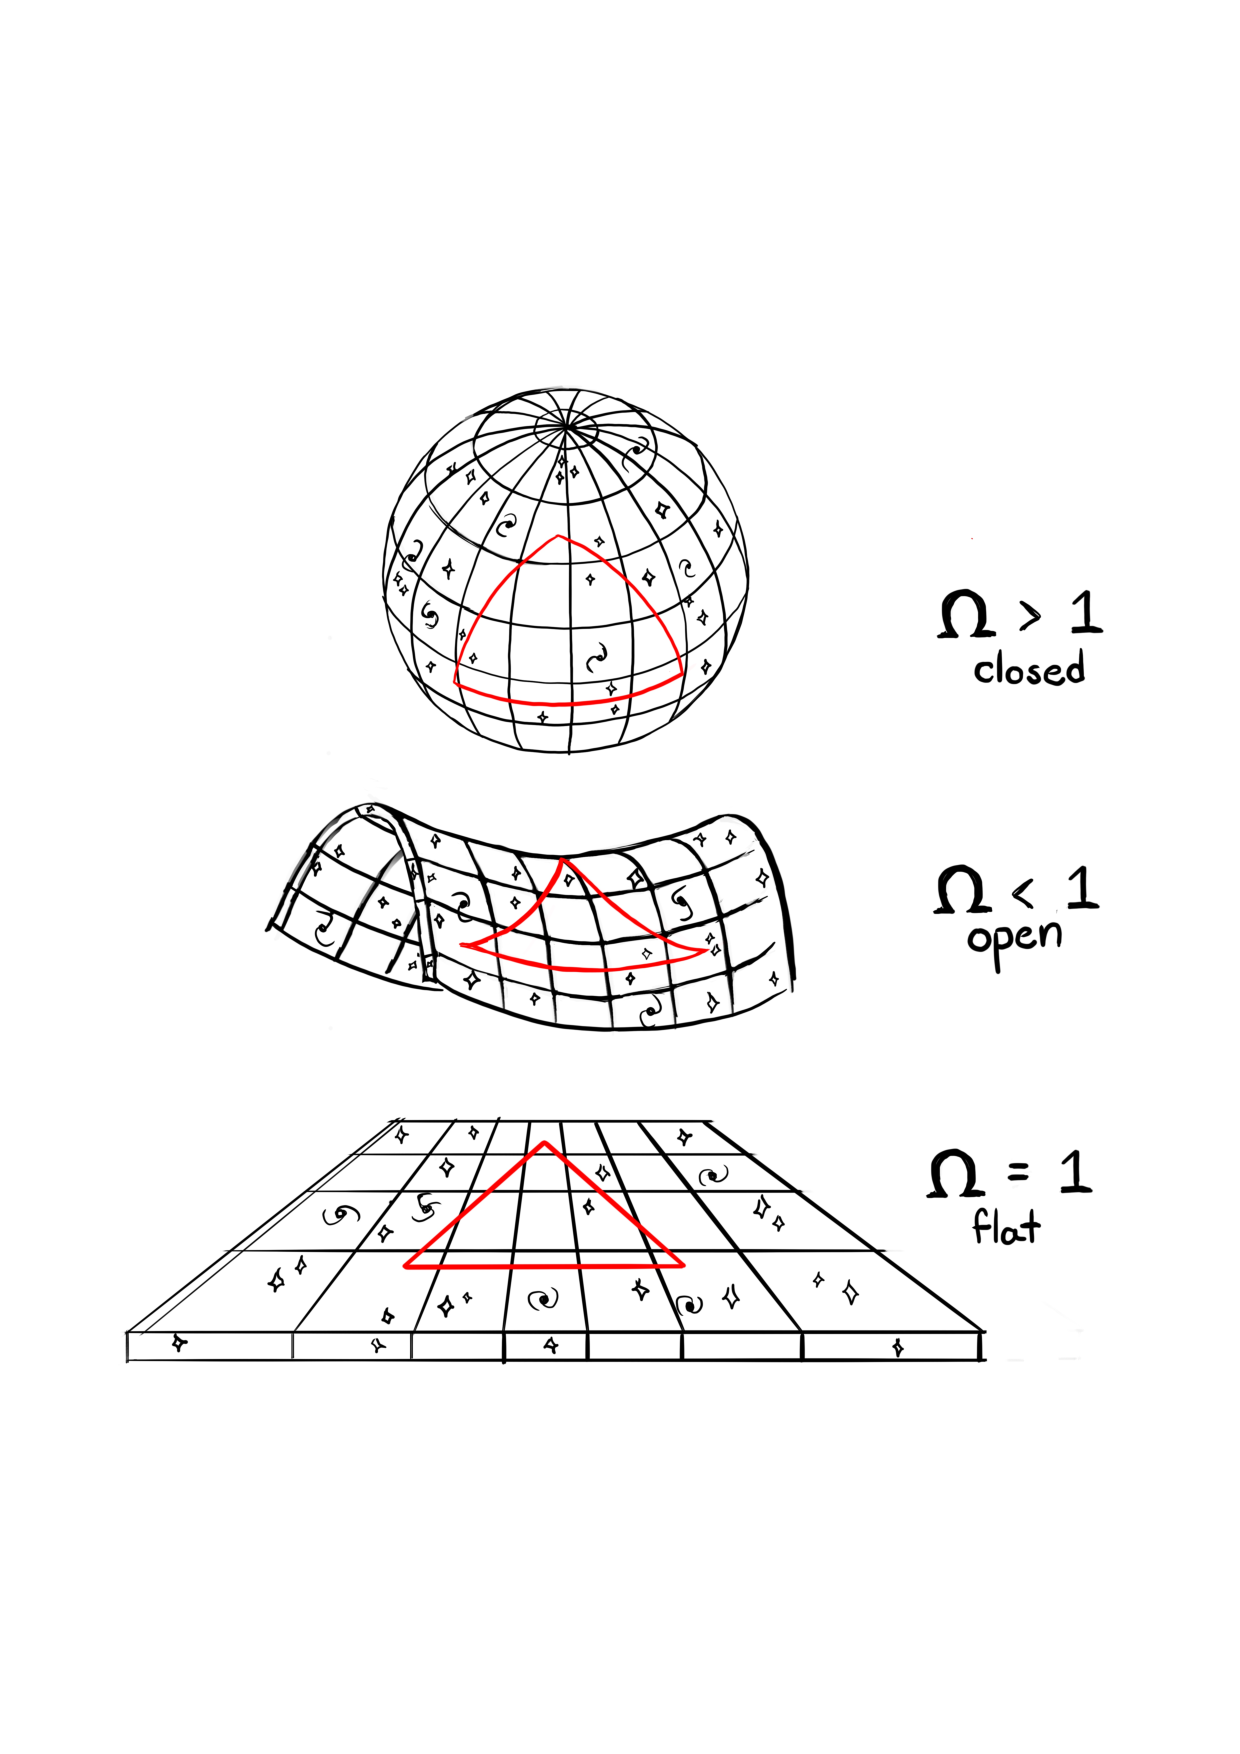
\includegraphics[width=\columnwidth]{Intro-FIGS/universeGeometry}
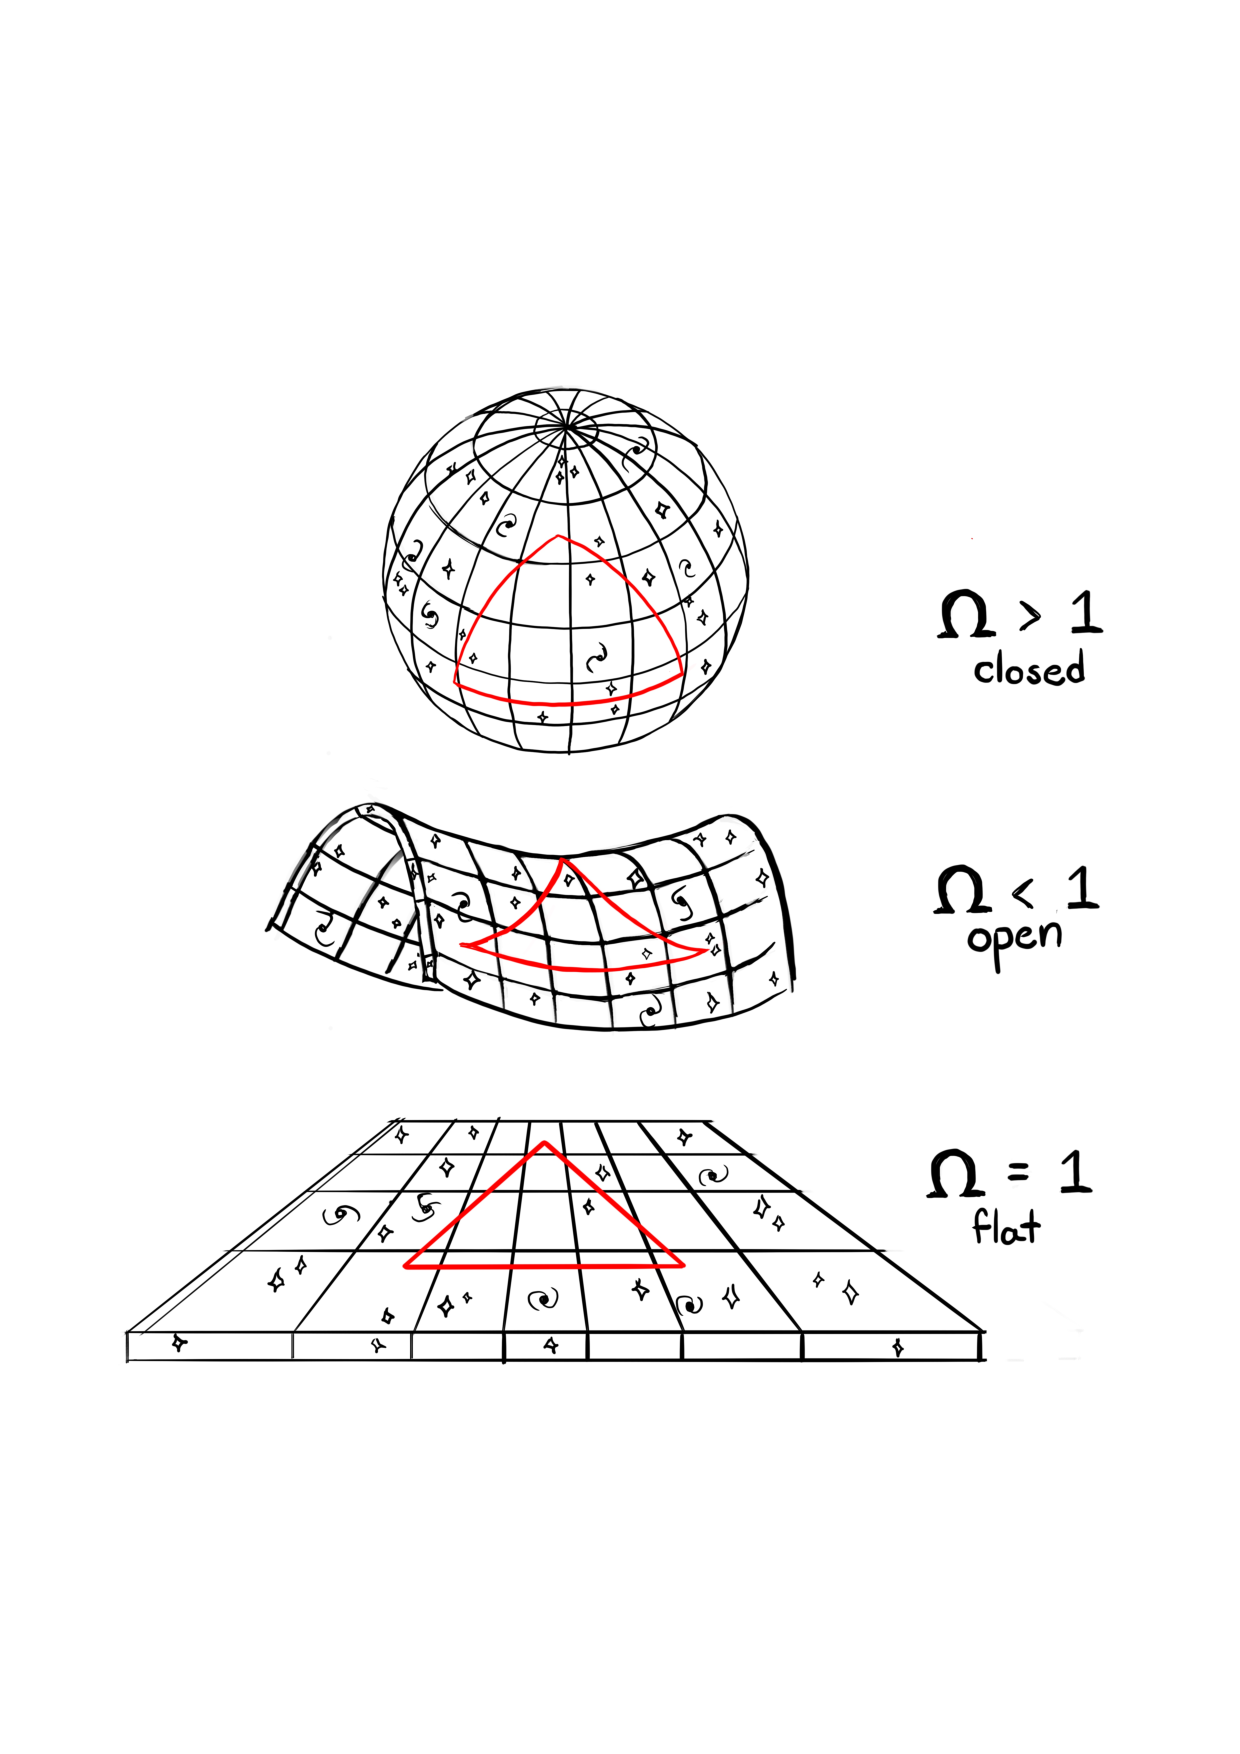
\includegraphics[width=\textwidth]{Intro-FIGS/universeGeometry}
\caption[Artistic representation of the geometry of the Universe and its matter-energy content. Figure created by R. Jackson.]{An artistic representation of the three geometries considered in the FRW metric -- Equation \eqref{Eq:Intro:FRW2} -- and their relationship between the total density of the Universe and the critical density, the dimensionless density parameter $\Omega \equiv \rho/\rho_c$. \textit{(top)} If $K = 1$ in Equation \eqref{Eq:Intro:Sk}, the total density is bigger than the critical density ($\Omega > 1$) and the geometry of the Universe is \textbf{closed}, meaning that the sum of internal angles of a 2D triangle is $> 180^o$. \textit{(middle)} If $K = -1$, total density of the Universe is smaller than the critical density ($\Omega < 1$) and the geometry of the Universe is \textbf{open} -- sum of internal angles of the 2D triangle is $< 180^o$. \textit{(bottom)} The last case happens when $K = 0$, when the total density of the Universe is precisely the critical density ($\Omega = 1$), this leads to a \textbf{flat} geometry for the Universe -- the usual Euclidean case, with the sum of internal angles of a triangle being precisely $180^o$. (Figure created by R. Jackson)}
\label{fig:Intro:Geometry}
\end{center}
\end{figure}

\subsubsection{Cosmological redshift}
Following the discovery made by \cite{1929Hubble}, nearby galaxies in the local Universe obey a linear law relating their distance and the rate at which they are distancing from a observer: $v = H_0x$. This relation is also known as \textbf{Hubble-Lema\^itre law}\footnote{Recently, during the 30th Meeting of the International Astronomical Union (IAU) in Vienna, the astronomical community decided to change this relation from `Hubble's law' to `Hubble-Lemaître law' \citep{2018IAU-HubbleLemaitre}.} -- where $H_0$ is referenced in modern cosmology as the \textbf{Hubble constant}. From the FRW metric, the physical distance between two fundamental observers (observers at rest in relation to the expansion of the Universe) is $a(t)dr$. Using this relation, Hubble's law can be re-written in a more generic fashion as 
\begin{equation}
H(t) = \frac{\dot{a}(t)}{a(t)}\, ,
\end{equation}
where the dot denotes a temporal derivative. 

\qquad At small scales, one can define the cosmological redshift in terms of the ration between the wavelength at the source of light and the observed light wavelengths,
\begin{equation}
\frac{\lambda_{\text{obs}}}{\lambda_{\text{source}}}  \equiv 1 + z\, ,
\end{equation}
where $z$ is the cosmological redshift as usually referenced in the literature. 

\qquad A general definition can be achieved when one considers a photon's null geodesic (in the absence of external forces or gravitational fields). As photons propagate radially in a geodesic, the FRW metric leads to 
\begin{equation}
r = \int \frac{dt}{a(t)}.
\end{equation}
Following, the comoving distance should be the same for all fundamental observers, therefore the integral above leads to
\begin{equation}
\frac{dt_{\text{source}}}{dt_{\text{obs}}} = \frac{a(t_{\text{source}})}{a(t_{\text{obs}})}.
\end{equation}
A conclusion here is that there is a time-dilation for photons emitted at distant galaxies which is proportional to the expansion of the Universe. This effect is reflected, as expected, in the observed wavelength yielding
\begin{equation}
\frac{1}{a(t)} = \frac{\lambda_{\text{obs}}}{\lambda_{\text{source}}}  \equiv 1 + z \, ,
\end{equation}
where, in the present time, $t_0$, it is defined as $a(t_0) = 1$. 

\qquad The ability to link the wavelength of light to the expansion of the Universe is a core concept in modern cosmology. As an example, it facilitates measurements of distance in the radial direction using spectra from spectroscopic surveys, or through the redshifted line-breaks of some types of galaxies through photometric bands' filters in photometric surveys \citep{AbdallaPhotoZ2011,2018-redshift}.

%%%%%%%%%%%%%%%%%%%%%%%%%%%%%%%%%%%%%%%%%%%%%%%%%%%%%%%%%%%
%					LCDM PARADIGM
%%%%%%%%%%%%%%%%%%%%%%%%%%%%%%%%%%%%%%%%%%%%%%%%%%%%%%%%%%%

\subsection{The $\Lambda$CDM Paradigm}\label{Sec:Intro:LCDM}
In the previous section, a relationship between geometry and the energy density content of the Universe appeared, relating $\Omega$ and $K$. In pursuance of a standard model for cosmology, the right hand side of Einstein's field equations, the energy-momentum tensor, needs to be defined. As this object must also obey the Cosmological Principle, it needs to be isotropic and homogeneous; a \textbf{perfect fluid} is a suitable candidate to describe the Universe in large scales. The energy-momentum tensor for a perfect fluid can be written as
\EQ{Intro:Tmunu1}{
T^{\mu\nu} = (\rho + p)\frac{dx^{\mu}}{ds}\frac{dx^{\nu}}{ds} - g^{\mu\nu}p,
}
where $\rho$ is the energy density and $p$ is the pressure exerted by the fluid. The expression from Equation \eqref{Eq:Intro:Tmunu1} can be re-written in comoving coordinates as
\EQ{Intro:Tmunu2}{
T^{\mu}_{\ \ \nu} = \left( \begin{array}{cccc}
-\rho & 0 & 0 & 0 \\
0 & p & 0 & 0 \\
0 & 0 & p & 0 \\
0 & 0 & 0 & p\end{array} \right).
}

\qquad Inserting the energy-momentum tensor above with the FRW metric into Einstein's field equations, one finds the dynamical equations governing the behaviour of the scale factor. First, one obtains the non-trivial components of the Einstein tensor as
\EQ{Intro:EFE_LCDM}{
G_{00} & = \frac{3}{a^2}\left( \dot{a}^2 + K \right) \, , \\
G_{ij} & = \frac{1}{a^2}\left( 2a\ddot{a} + \dot{a}^2 + K \right)\delta_{ij},
}
where $\delta_{ij}$ is the Kronecker delta. Next, including the energy-momentum tensor from Equation \eqref{Eq:Intro:Tmunu2}:
\EQ{Intro:Fried1}{
\left(\frac{\dot{a}}{a}\right)^2 & = \frac{8\pi G}{3}\rho - \frac{K}{a^2} + \frac{\Lambda}{3}\, ,}
and
\EQ{Intro:Fried2}{
\frac{\ddot{a}}{a}&  = -\left\lbrace 4\pi Gp + \frac{1}{2}\left[\left(\frac{\dot{a}}{a}\right)^2 + \frac{K}{a^2}\right] \right\rbrace + \frac{\Lambda}{3}\, .
}

\qquad These are known as the Friendmann Equations \citep{1922Friedmann}, combining them leads to
\EQ{}{
\frac{\ddot{a}}{\dot{a}} = -\frac{4\pi G}{3}(\rho + 3p)\, ,
}
which implies that the acceleration is independent of the geometry, $K$. However, one can re-write Equation \eqref{Eq:Intro:Fried1} to obtain an expression for $K$ in terms of the time dependent variables $a(t)$, $\rho (t)$, and $p(t)$ \citep{padmanabhan_1999}. At the present time, $a(t=t_0) = 1$, 
\EQ{Intro:K}{
K & = \frac{8\pi G}{3} \rho (t_0) - \dot{a}^2(t_0) + \frac{\Lambda}{3} \\
& \equiv  H_0^2(\Omega(t_0) - 1)\, ,
}
here, $H_0$ is the Hubble constant measured today and $\Omega \equiv \rho/\rho_c$ is again the dimensionless total density of the Universe. The critical density, $\rho_c$, is defined to be the precise energy density the Universe needs so its geometry is flat, i. e. $K=0$; it can be defined from Equation \eqref{Eq:Intro:K} as $\rho_c \equiv 3H_0^2/8\pi G = 8.098 \times 10^{-11} \text{eV}^{4}$. Figure \ref{fig:Intro:Geometry} shows the relationship between the total density of the Universe and its geometry.

\qquad It is useful to express Equation \eqref{Eq:Intro:Fried2} in terms of the Universe's components and their evolution according to the scale factor: pressureless matter (baryonic or dark), $\rho_m = (\rho_{b} + \rho_{cdm}) \propto a^{-3}(t)$; radiation, $\rho_r \propto a^{-4}(t)$; and vacuum energy, $\rho_{\Lambda} = \Lambda/8\pi G$. Using these relations, the second Friedmann equation -- Equation \eqref{Eq:Intro:Fried2} -- can be expressed in terms of the Hubble constant

\EQ{Intro:HubbleOmega1}{
E^2(t) \equiv \frac{H^2(t)}{H_0^2} = \left[ \Omega_r a^{-4}(t) + \Omega_m a^{-3}(t) + \Omega_K a^{-2}(t) +  \Omega_{\Lambda} \right], 
}
where the $\Omega_i$ are the dimensionless density of each component $i$ considered
\EQ{}{
\Omega_r \equiv \frac{\rho_r(t_0)}{\rho_c} \, ; \quad \Omega_m \equiv \frac{\rho_m(t_0)}{\rho_c} \, ; \quad \Omega_{\Lambda} \equiv \frac{\rho_{\Lambda}}{\rho_c} \, ; \\ 
\Omega_K \equiv 1 - (\Omega_r + \Omega_m + \Omega_{\Lambda}) = 1 - \Omega \, .
}
Promtly, Equation \eqref{Eq:Intro:HubbleOmega1} can be written in terms of the equation-of-state, $w_i$, for each of the components
\EQ{Intro:HubbleOmega2}{
E^2(t) & = \sum_i \Omega_i a^{-3(1+w_i)} \\
	& = \sum_i \Omega_i(1+z)^{3(1+w_i)}
}
with
\EQ{Intro:EoS}{
w_i = 
\begin{cases}
1/3, & \text{for radiation} \\
0, & \text{for matter (dark and baryonic)} \\
-1/3, & \text{for curvature}\\
-1, & \text{for vacuum or cosmological constant}
\end{cases}
}

\qquad Now, the comoving distance at a given redshift can simply be expressed as
\EQ{Intro:Comoving}{
\chi (z) = \frac{1}{H_0}\int_0^z \frac{dz'}{E(z')}
}
which means that distance measurements in comoving coordinates depend on the energy density content of the Universe at a given redshift. 

\qquad A brief description of each of the components of the Universe follows in the next subsections \citep{dods,schneider_2016}.

\subsubsection{Radiation, $\Omega_r$ :}
 Cosmic microwave background experiments such as COBE \citep{COBE}, WMAP \citep{WMAP_MapsResults,WMAP_Cosmology}, and the Planck Satellite \citep{2018PlanckCosmology} all measure the temperature of the CMB photons. The CMB photon temperature has been measured with incredible precision already with the FIRAS instrument (on-board of the COBE satellite) to be a perfect fit of a black-body radiation with $T_{cmb} = 2.725\pm 0.002$K \citep{1999FIRAS}. The energy density of photons can be estimated from statistical mechanics using the Bose-Einstein distribution function \citep{dods}
 \EQ{Intro:CMB:Temp}{
 \rho_{\gamma} & = 2\int \frac{d^3p}{(2\pi)^3} p \left( e^{p/T_{cmb} -1 }\right)^{-1} \\
 	& = \frac{\pi^2}{15}T_{cmb}^4 \\
    & = \frac{\pi^2}{15}\left( \frac{2.725 K}{a} \right)^4
 }
and the equation-of-state for radiation is consistent with the pressure exerted by this component, $p_r = \frac{1}{3}\rho_r$. In terms of the dimensionless radiation density, $\Omega_r \approx 5 \times 10^{-5}$ \citep{schneider_2016}.

\qquad Part of the radiation content is also composed of neutrinos, even thought the mass of these particles are small, it is known that it is non-zero \citep{Kamiokande1998}. Neutrinos, therefore, act relativistically at decoupling causing them to behave as radiation in the early Universe.

\begin{figure}
\begin{center}
%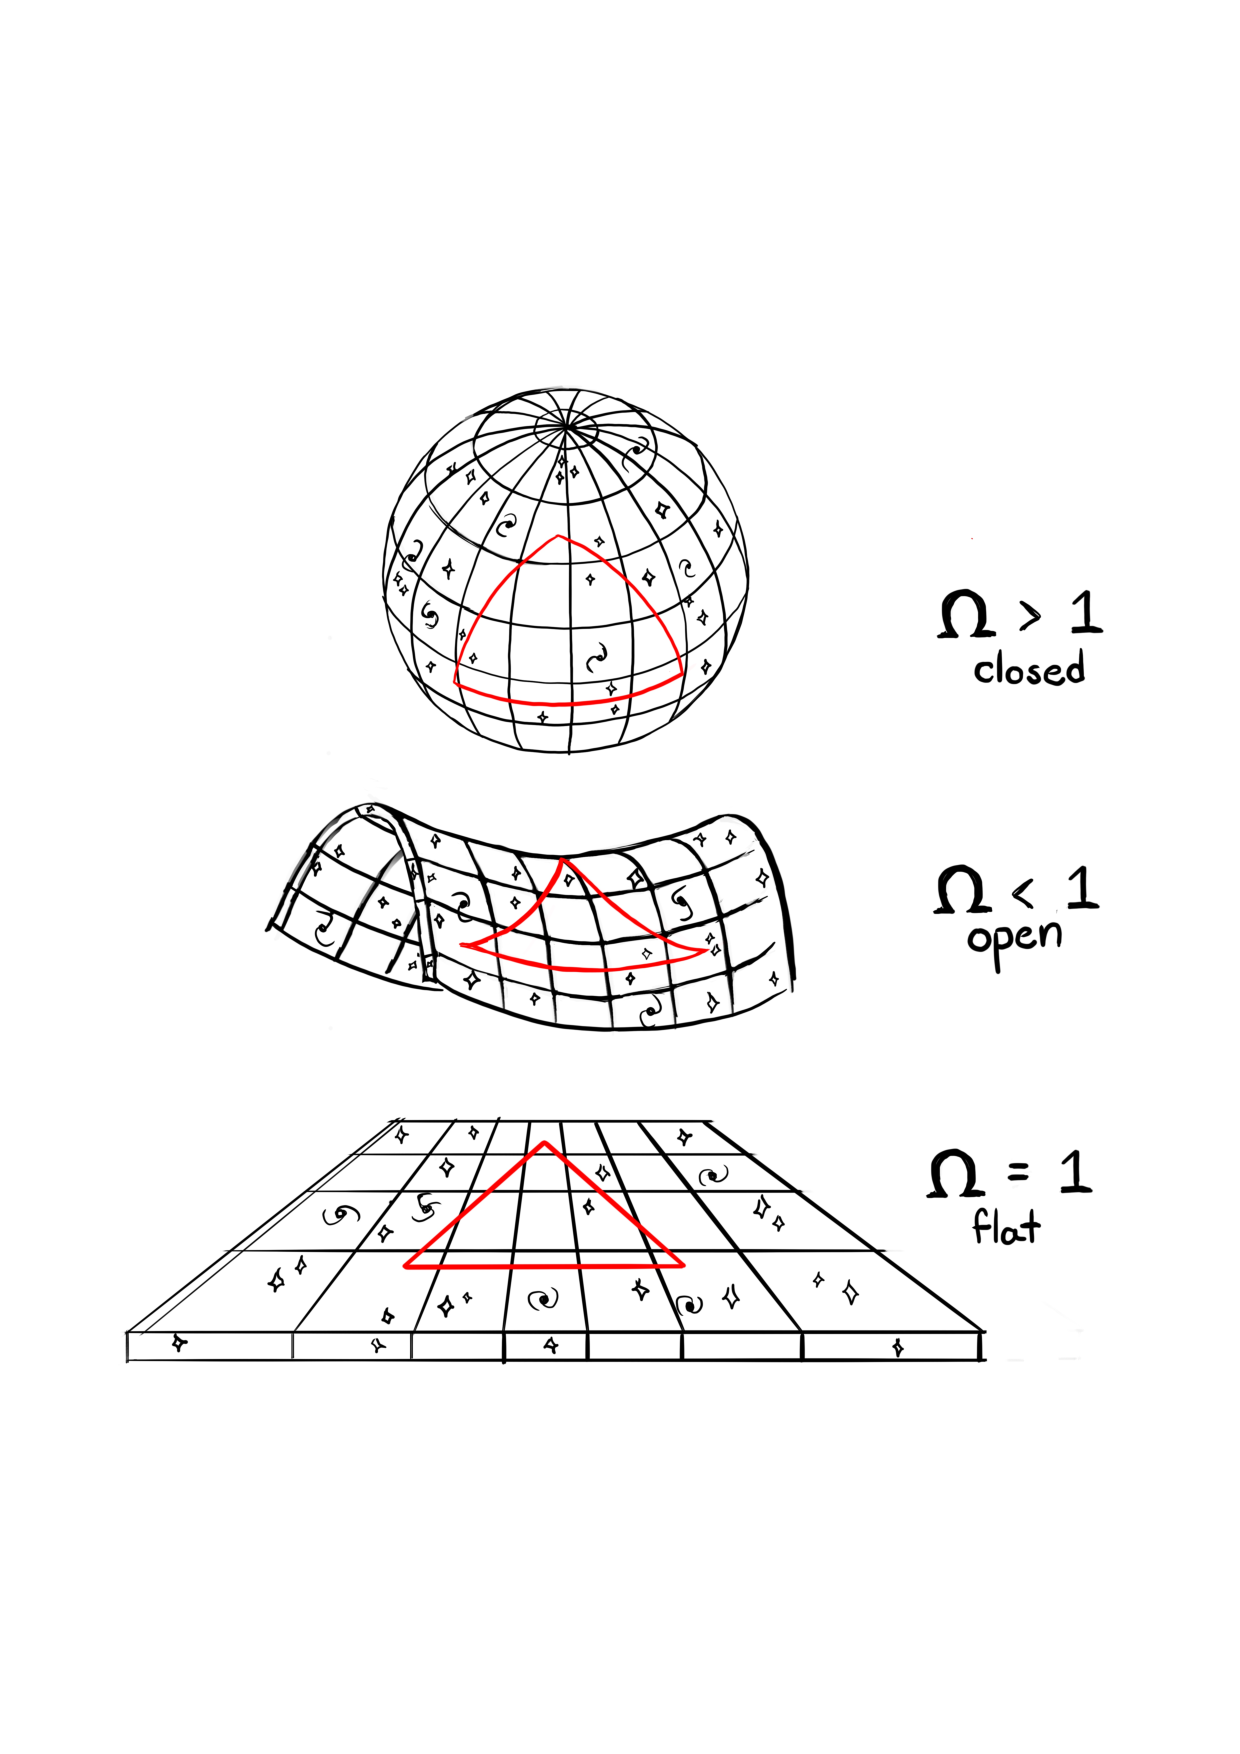
\includegraphics[width=\columnwidth]{Intro-FIGS/universeGeometry}
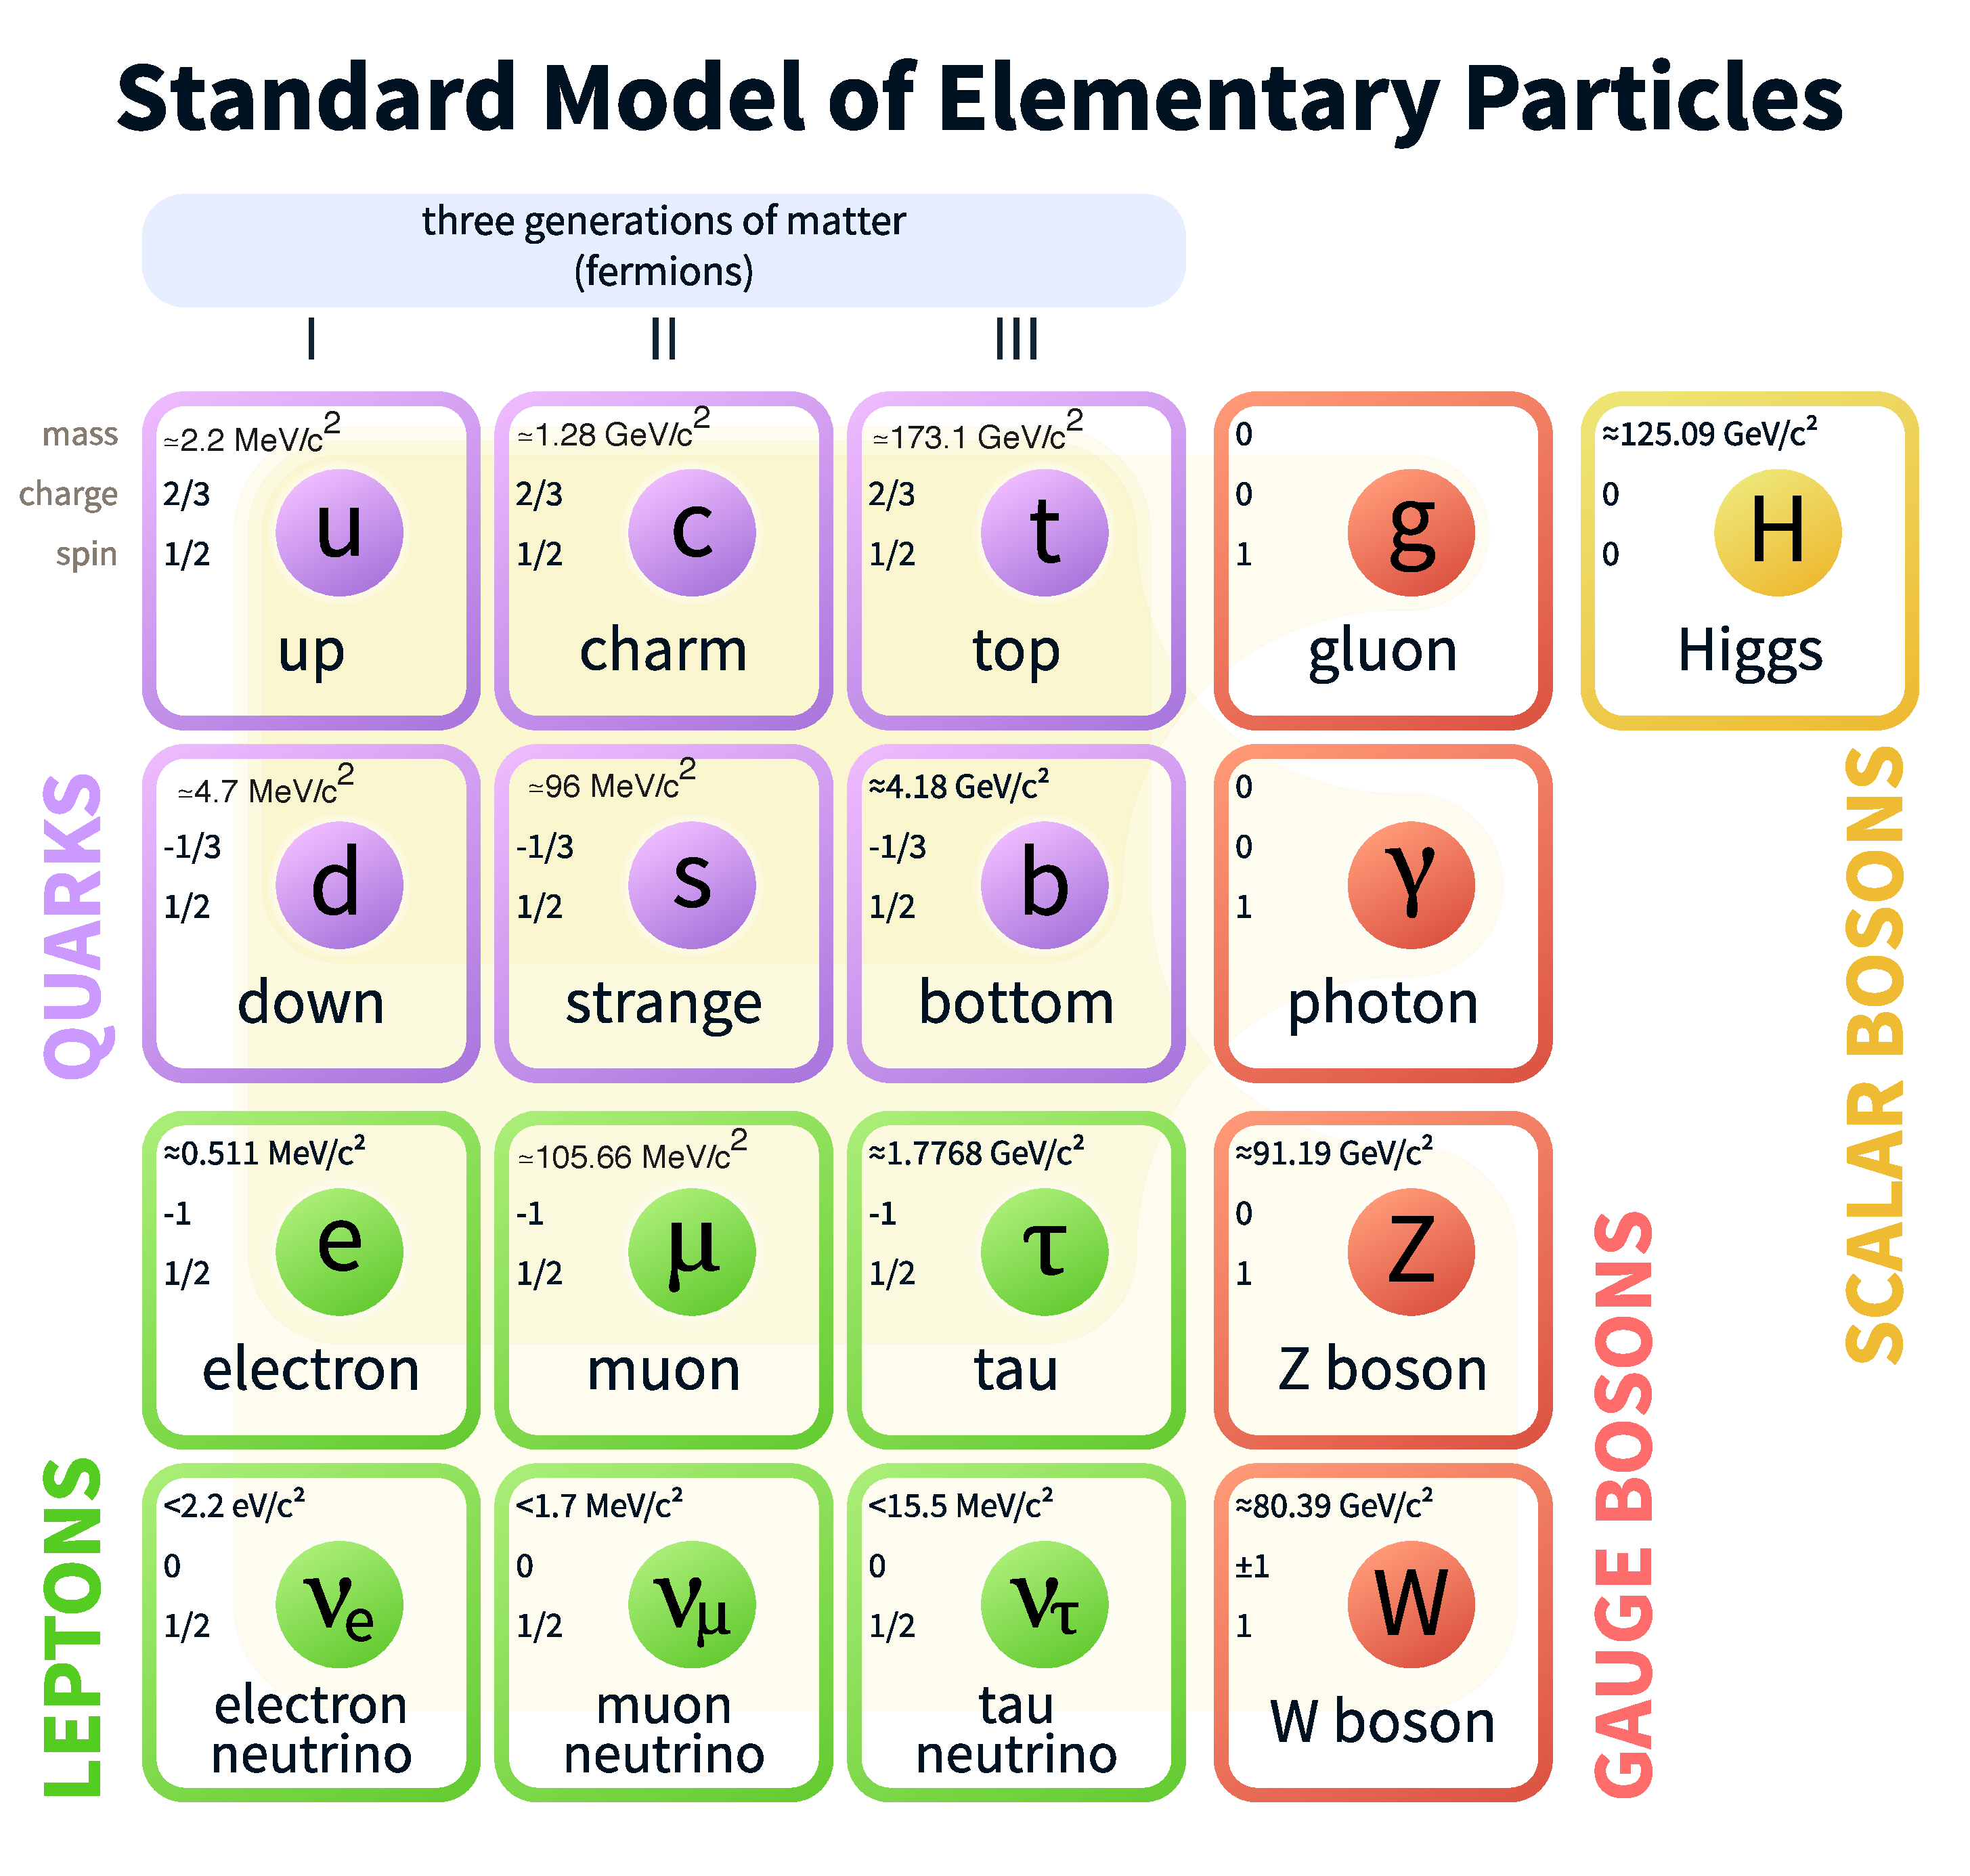
\includegraphics[scale=0.30]{Intro-FIGS/standard_model}
\caption[Standard Model of Particle Physics. (Source: Particle Data Group -- \url{http://pdg.lbl.gov})]{Standard Model of Particle Physics: \textit{(purple)} the six quarks; \textit{(red)} the four gauge bosons: gluon (strong force), photon (electromagnetic force), Z and W bosons (weak force); \textit{(green)} the six leptons: the three neutrino species and their charged counterparts; \textit{(yellow)} the newly experimentally discovered Higgs bosons, a scalar boson. All of these particles, with the exception of the W boson and the photon, have their associated anti-particle. The top values in the neutrino boxes show the upper bounds for each flavour's mass. (Source: Wikipedia, Particle Data Group -- \url{http://pdg.lbl.gov})}
\label{fig:Intro:StandardModel}
\end{center}
\end{figure}

%%%%%%%%%%%%%%%%%%%%%%%%%%%%%%%%%%%%%%%%%%%%%%%%%%%%%%%%%%%
%					ENERGY CONTENT
%%%%%%%%%%%%%%%%%%%%%%%%%%%%%%%%%%%%%%%%%%%%%%%%%%%%%%%%%%%

\subsubsection{Baryonic Matter, $\Omega_b$ :}
Baryonic matter constitutes all matter as we commonly refer to: all the atoms in the periodic table, electrons, neutrons, protons and more. In other words, any sort of particles described by the Standard Model of Particle Physics (Figure \ref{fig:Intro:StandardModel}) -- apart from neutrinos which, even though being massive, behave close to being relativistic in the early Universe. The baryonic matter density behaves similarly to a gas with a certain temperature but with zero chemical potential. Baryons interact with other components not only via gravitational interaction but also via the electromagnetic force. Therefore, baryons and photons are coupled throughout the history of the Universe; during this phases, baryonic matter has an equation-of-state $p = \rho/3$. After photons and baryons decouple, this component behaves as a pressureless fluid with an equation-of-state $p=0$. 

\qquad In a seminal work by \cite{1998BaryonContent}, the authors estimate the baryonic content of the Universe using four different methods at low redshift ($z \approx 0$), high redshift ($z\approx 3$) gas components, and big bang nucleosynthesis (BBN) abundances \citep{2000-BBN-Review,2016R-BBN-Review}. The low redshift indicators contain stars in elliptical, spiral, and irregular galaxies, neutral atomic gas, plasma in clusters, warm and cool plasma in the intermediate mean in cluster groups -- with a sum of $\Omega_b = 0.021$. High redshift indicators constitute damped absorbers and Ly$\alpha$ forest clouds \citep{2003Weinberg-Lyalpha}, representing a value of $\Omega_b$ agreeing with the low redshift measurements. From BBN, the abundances of Deuterium and Helium also indicate a baryonic content of $\Omega_b \approx 0.021\pm 0.007$. These values are consistent with the current value found by \cite{2018PlanckCosmology} ($\Omega_b h^2 = 0.0224 \pm 0.0001$) and the values found in BOSS analysis in Chapter \ref{Chap:BOSS-Cosmo}.

\subsubsection{Cold Dark Matter, $\Omega_{cdm}$:}
Cold dark matter is inferred indirectly via several observations -- including the rotational curves of galaxies \citep{1970Rubin} and gravitational lensing measurements in galaxy clusters \citep{2006BulletCluster} -- indicating that the majority of matter in the Universe is electromagnetically non-interactive, non-relativistic, and non-luminous. This strange component interacts only gravitationally and, as a consequence, it is not coupled to photons. This causes dark matter to start clustering earlier than baryonic matter. As there is no coupling, this component also behaves as a pressureless fluid, $p_{cdm} = 0$, since very early in the Universe. The correlation function of galaxies \citep{Einsenstein2005}, the power spectra of galaxies \citep{Blake2007,BOSS}, and the CMB acourstic peaks \citep{PlanckCosmology2016,PlanckResults2015,2018PlanckCosmology} also need the additional existence of cold dark matter in order to explain the baryon acoustic oscillation (BAO) peak and other features of the 2-point statistics in the analysis (see Section \ref{Sec:Intro:Pk}). These measurements combined seem to suggest that $\Omega_{cdm} \approx 0.25$ .

\qquad Empirical evidence for cold dark matter comes only through indirect gravitational observations, no direct detections were made so far \citep{2017DarkMatterExpReview}. In light of these null detections, there are some attempts to explain it with alternative theories. In the early years, neutrinos were a good candidate for dark matter as they interact very weakly via the electromagnetic field. Although, this hypothesis was later discarded as they later proved to behave more as a hot dark matter -- washing away structure instead of forming it earlier as CDM. Some other alternative theories came from questioning the nature of GR, like Modified Newtonian Dynamics (MOND, \citealt{1983MOND}). MOND tries to explain the observational effects attributed to cold dark matter by introducing an acceleration scale in which Newtonian dynamics is modified. Even though it was created in order to solve the observations explained by dark matter, there are several issues with this theory where it fails to explain other dark matter observations \citep{2011MondSucks}. One of them, claimed as `a direct empirical proof of the existence of dark matter' by \cite{2006BulletCluster} can only be explained by MOND if the sum of mass of neutrinos were $\sum m_{\nu} \approx 2.0$ eV \citep{2007ApJ...654L..13A}. Such value is already excluded by galaxy clustering measurements -- \citealt{Thomas2010Neutr,2014Gonzalez-GarciaNeutrino} as well as measurements shown in Chapters \ref{Chap:BOSS-Cosmo} and \ref{Chap:Neutrinos} -- which makes MOND very unlikely to be true.  

\subsubsection{Cosmological Constant or Dark Energy, $\Omega_{\Lambda}$ or $\Omega_{de}$:}
Observations of Supernovae type Ia luminosity distance relation strongly suggest that something is causing the Universe to go through an accelerated expansion phase \citep{1998Riess,1999Perlmutter,2018LambdaCentury}. The furthest away galaxies are, the faster they distance themselves from each other. This effect is attributed to a mysterious component called dark energy which seems to compose around $70\%$ of the Universe \citep{2018PlanckCosmology}. This component seems to exert a negative pressure, $p_{de} \leq - \frac{1}{3}\rho_{de}$; it can be parametrised in terms of the equation-of-state parameter, $w_0$ -- where, if $w_0 = -1$, dark energy is simply the cosmological constant, $\Lambda$, as $p_{\Lambda}= -\frac{1}{3}\rho_{\Lambda}$. Any deviation from $w_0 = -1$ would mean new physics, beyond the standard $\Lambda$CDM model. Current observations from the Dark Energy Survey combined with BAO measurements from BOSS \citep{2016BOSSCosmology}, and CMB from Planck \citep{PlanckCosmology2016} seem to suggest that $w_0 = -1.00^{+0.04}_{-0.05}$. Measurements shown in Chapter \ref{Chap:BOSS-Cosmo} are consistent with the DES findings; these seem to suggest that dark energy is simply the cosmological constant, $\Lambda$. A lot of questions are still unanswered in Cosmology as the nature of $\Lambda$ is still unknown -- if one does not accept it as a fundamental property of spacetime.

\subsubsection{Neutrinos, $\Omega_{\nu}$:}
Produced by weak force interactions, neutrinos come in three different leptonic flavours: neutrino electron ($\nu_e$), neutrino muon ($\nu_{\mu}$), and neutrino tau ($\nu_{\tau}$); which are all associated with their corresponding charged leptons: electron, muon, and tau (see Figure \ref{fig:Intro:StandardModel}). As mentioned before, experiments in the late 90s like the Super Kamiokande \citep{Kamiokande1998} and subsequent experiments \citep{2002SNO,2005KamLAND,2008MINOS,2012RENOExperiment,AbeNeutrino2014} demonstrated that neutrinos oscillate between flavours which was a smoking gun to the theory that neutrinos have finite mass eigenstates. The total mass of neutrinos and their hierarchy (or ordering) is still unknown as particle physics oscillation experiments can only measure the square mass splitting between species \citep{2014Gonzalez-GarciaNeutrino}:
\begin{align}
\Delta m_{21}^2 & \equiv m_2^2 - m_1^2 \nonumber \\ 
				& \approx 7.49^{+0.19}_{-0.17} \times 10^{-5}\, \text{eV}^2 \label{Eq:Intro:Mass21}
\end{align}
\begin{align}
|\Delta m_{31}|^2 & \equiv |m^2_3 - m_1^2| \nonumber \\ 
				  & \approx 2.484^{+0.045}_{-0.048} \times 10^{-3} \, \text{eV}^2. \label{Eq:Intro:Mass31}
\end{align}
The measurement in Equation \eqref{Eq:Intro:Mass21} comes from solar neutrino oscillation experiments, while the measurement in Equation \eqref{Eq:Intro:Mass31} comes from atmospheric neutrino oscillation experiments. Both these measurements imply that at least two of the neutrino species have a non-zero mass. However, as the signal in the $|\Delta m_{31}|^2$ is unknown, two different hierarchies are possible if the masses are not completely degenerate.

\qquad The large scale structure of the Universe is sensitive to the sum of neutrino mass species, $\sum m_{\nu} = m_1 + m_2 + m_3$, as the cosmic neutrino density can be probed via the dimensionless density of neutrinos, $\Omega_{\nu} \propto \sum m_{\nu}$. In the early Universe, when the neutrino temperature was sufficiently high, the energy density of neutrinos is related to that of photons (Equation \ref{Eq:Intro:CMB:Temp}) as %$\Omega_{\nu} \approx \sum m_{\nu}/(93.14h^2 \, eV)$ \citep{dods}. 

\EQ{Intro:NuRho1}{
\rho_{\nu} = \frac{7}{8}\left( \frac{4}{11}\right)^{3/4}\rho_{\gamma}
}
where the factors in the above equation are related to the degeneracy factor of neutrinos, the fact that neutrinos are fermions and obey a Fermi-Dirac distribution which leads to a factor of $(4/11)^{1/3}$, and, finally, the energy density of massless particles scaling with temperature with $T^{4}$ for photons \citep{dods}. For massive neutrinos, Equation \eqref{Eq:Intro:NuRho1} can be expressed as 
\EQ{}{
\rho_{\nu'} = \frac{2}{(2\pi)^3}\int d^3p \frac{\sqrt[]{p^2 + (m_{\nu'})^2}}{e^{p/T_{\nu'}}+1}.
}
for each individual neutrino species, $\nu'$. After the neutrino temperature ($T_{\nu'}$) drops to $T_{\nu'} \sim  m_{\nu'}$, massive neutrinos start behaving non-relativistically and their overall contribution to the energy density content of the Universe is \citep{2003HannestadNeutrino}

\EQ{}{
\Omega_{\nu} \approx \frac{\sum m_{\nu}}{92.5h^2 \text{eV}}
}


\qquad Still, massive neutrinos act as some sort of ``warm dark matter" as they are almost relativistic while barely interacting with matter other than gravitationally -- this means that massive neutrinos tend to ``wash away'' structure in smaller scales. In \cite{2003HannestadNeutrino}, and more recently in \cite{2016JCAP...11..035H}, the authors demonstrate the case for measuring not only the upper limit for $\sum m_{\nu}$, but also the neutrino mass hierarchy from cosmological galaxy surveys. In Chapter \ref{Chap:Neutrinos}, I explore the impact of modelling the neutrino mass and neutrino mass hierarchy using different assumptions and datasets.


\subsubsection{Curvature, $\Omega_K$:}
As shown in Equation \eqref{Eq:Intro:K} and Figure \ref{fig:Intro:Geometry}, there is a direct relationship between the curvature of the Universe, its energy content, and the critical density, $\rho_c$. If $\Omega = 1$, the Universe is perfectly flat with $K=0$. Recent results from the Planck collaboration observations estimate $\Omega_K = 1 - \Omega = 0.0007\pm 0.0037$ \citep{2018PlanckCosmology}. This is a very strong observational evidence that the Universe is flat, meaning that the energy density of the Universe is precisely the critical density with 0.2\% accuracy. 

\vspace{5mm}

\qquad In summary, the $\Lambda$CDM background Universe can simply be described by a FRW metric, a perfect fluid, and the cosmological constant. The standard cosmological model implies that our Universe is going through an accelerated expansion phase in the present time, i. e. it is currently dominated by the cosmological constant, and contains a flat geometry. Distances are measured related to the scale factor, $a(t)$, which, according to the FRW metric evolves with time. Finally, the baryonic content of the Universe is insufficient to describe several cosmological and astrophysical observations, leading to the necessity of dark matter to explain these phenomena. 

\qquad There are still several pieces missing in the $\Lambda$CDM paradigm puzzle, the main ones being \textbf{the horizon problem} and the \textbf{flatness problem} \citep{1994Hu-Flatness-Horizon,2005Lake-PRL-Flatness,2012Helbig-flatness}. The first one, the horizon problem, is related to the thermalisation of photons in the CMB. Since signals can't travel faster than the speed of light, CMB photons separated by more than one degree in the sky should have originated from completely uncorrelated parts of the very early Universe. These means that no information, like temperature, between such regions could have been exchanged. This, however, is not what is observed in the cosmic microwave background. Fluctuations in the CMB temperature are of the order of $\Delta T/T \sim 10^{-5}$. The second issue, the flatness problem (also known as the coincidence problem), is related to the extreme coincidence that our Universe has precisely the energy density needed for it to be flat, i. e. $\Omega = 1$. For this to happen, a very careful ``fine-tuning'' in the early Universe's parameters was necessary. Although theories like \textbf{inflation} claim to solve both these issues (see \citealt{2008InflationReview} for a review), no cosmological observations seem to confirm even the simplest of predictions from inflation \citep{2014Bicep2Planck}.

\vspace{10mm}
%%%%%%%%%%%%%%%%%%%%%%%%%%%%%%%%%%%%%%%%%%%%%%%%%%%%%%%%%%%
%				INHOMOGENEOUS UNIVERSE
%%%%%%%%%%%%%%%%%%%%%%%%%%%%%%%%%%%%%%%%%%%%%%%%%%%%%%%%%%%
\section{Probing inhomogeneities in the Universe}
During the last section, I described the Universe at extremely large scales -- the background Universe. However, when observed in `not so large scales', structures like groups of galaxies, clusters, filaments, voids, and more appear. This demonstrates that at certain scales the Universe's behaviour is dominated by these inhomogeneities. The accelerated expansion of the Universe, combined with the attractive nature of gravity creates structures like groups and clusters of galaxies which are not randomly distributed in the sky. Rather, positions in the sky of such objects are correlated in a way that depends on the matter-energy density, geometry, and content of the Universe. This section will explore how to understand the Universe using the statistical distribution of galaxies and other probes of inhomogeneity.

\qquad Since the first galaxy redshift surveys, structures like the Great Wall \citep{SloanGreatWall} and the Great Attractor \citep{ScharfLahav1992} appeared in the distribution of galaxies indicating that much can be understood about the Universe by probing these inhomogeneities. When combining this observations with the CMB temperature anisotropies ($\Delta T/T \sim 10^{-5}$), it becomes clear that anisotropies in the CMB where the seed to the formation of structures in the late Universe. 

%%%%%%%%%%%%%%%%%%%%%%%%%%%%%%%%%%%%%%%%%%%%%%%%%%%%%%%%%%%
%				INHOMOGENEOUS UNIVERSE
%%%%%%%%%%%%%%%%%%%%%%%%%%%%%%%%%%%%%%%%%%%%%%%%%%%%%%%%%%%
\subsection{Linear perturbation Theory}\label{Sec:Intro:LinTheory}
Any attempt to describe the distribution of matter in the Universe in a deterministic way, trying to model the precise location of each celestial object, would lead to frustration and failure. Instead, one should attempt to describe the statistical properties of the distribution of matter in the Universe, i. e. to statistically describe the matter density field. When probing the way matter behaves in the presence of gravity in an expanding Universe, the \textbf{matter overdensity field} is an important tool;  it can be defined as
\EQ{Intro:OverdContrast}{
\delta(\textbf{r},t) \equiv \frac{\rho(\textbf{r},t) - \bar{\rho}(t)}{\bar{\rho}(t)},
}
where $\bar{\rho}(t)$ is the mean matter density in a given time or redshift. Over time, density fluctuations grow due to the gravitational interaction with nearby matter: over-dense regions will become denser with time, increasing the overdensity field locally; while under-dense regions will become less dense. In other terms, the module of the matter overdensity field, $| \delta |$ increases as the Universe evolves.

\subsubsection{Perturbations on Boltzmann equations:}
To obtain the evolution of the matter overdensity field, one needs to solve a series of coupled differential equations taking into account the coupling and evolution of all components described in Section \ref{Sec:Intro:LCDM}. Linear perturbation theory is a widely spread method to solve problems of this nature in physics. Here, I will follow a similar path and description as the one presented in \cite{Peacock} and \cite{dods} in which one solves the Boltzmann equations for each of the components of the Universe using perturbation theory in a FRW background Universe. 

\qquad Starting with the collisional Boltzmann equation and the occupation function for each component, \textit{f}, 
\EQ{Intro:Boltzmann}{
\frac{df}{dt} = \frac{\partial f}{\partial t} + \frac{dx^i}{dt}\frac{\partial f}{\partial x^i} + \frac{d p}{dt}\frac{\partial f}{\partial p} = \mathcal{C}[f]
}
where $\mathcal{C}[f]$ accounts for any sort of collisions and coupling a component might experience throughout the evolution of the Universe.

\qquad The left hand side of Equation \eqref{Eq:Intro:Boltzmann} takes into account perturbations in the background FRW metric. Using the conformal Newtonian gauge \citep{dods}, the background metric can be described using two potentials with dependence on spacetime: $\Psi (\textbf{r}, t)$ and $\Phi (\textbf{r}, t)$. The non-vanishing terms in the perturbed metric are
\EQ{Intro:PertMetric_00}{
g_{00}(\textbf{r},t)=-(1+2\Psi(\textbf{r},t))
}
and 
\EQ{Intro:PertMetri_ij}{
g_{ij}(\textbf{r}, t) = a^2(t)(1+2\Phi(\textbf{r},t))\delta_ij
}
which, for a Universe with no anisotropic stress, leads to $\Psi (\textbf{r},t) = \Phi(\textbf{r},t)$ \citep{Peacock}. Equation \eqref{Eq:Intro:Boltzmann} can now be re-written as
\EQ{Intro:BoltzmannFinal}{
\frac{\partial f}{\partial t} +\frac{p\hat{p}_i}{a(t)E} \frac{\partial f}{\partial x^i}-\frac{\partial f}{\partial E}\left( \frac{p^2}{E}\dot{\Phi} + \frac{\partial \Psi}{\partial x^i}\frac{p\hat{p}_i}{a(t)} + \frac{p^2}{E}H(t)\right) = \left[ \frac{\partial f}{\partial t} \right]_{\mathcal{C}}\, ,
}
where E is the energy and p is the momentum with a unity directional vector $\hat{p}_i$ of a certain component of the Universe. This equation, together with the perturbed Einstein's field equations, describe fully the perturbation's evolution throughout the history of the Universe.

\qquad The Universe's components can be divided into two main categories: relativistic components -- like photons and neutrinos -- and non-relativistic components -- like dark and baryonic matter. Within the same category, components behave in a similar fashion; however, with different couplings. In Fourier space, the evolution of these components depends mainly on the magnitude of the wave-number vector ($k \equiv |\textbf{k}|$), the conformal time ($\eta$), and the angle between the k-modes and the momenta ($\mu\equiv \hat{k} \cdot \hat{p}$). 

\qquad The fractional temperature difference of photons, $\Delta T/T$, can be expressed in Fourier space as
\EQ{}{
\Theta(k,\mu,\eta) = \int d^3r\frac{\Delta T(\textbf{r},\eta)}{T(\textbf{r},\eta)}\exp\left( -ikr\mu \right)\, ,
}
which can be expanded using Legendre polynomials, $\mathcal{L}_{\ell}(x)$, in order to express the photons' temperature field in terms of the $\ell$-th multipole:
\EQ{}{
\Theta_{\ell} = \frac{1}{(-i)^{\ell}}\int_{-1}^{1} \frac{d\mu}{2}\Theta(\mu)\mathcal{L}_{\ell}(\mu)\, .
}
Higher multipole modes describe the small scale domain, while lower multipoles dominate the behaviour of photons in the Universe in larger scales. 

\qquad The other relativistic components of the Universe can be equally described; using a similar approach one can describe the neutrino density perturbations expressed by $\mathcal{N}(k,\mu,\eta)$. The non-relativistic components can be described by the overdensity field, $\delta_{cdm}(k,\eta)$ and $\delta_b(k,\eta)$ -- for dark and baryonic matter, respectively --, and their velocity fields in Fourier space, $v_{cdm}(k,\eta)$ and $v_{b}(k,\eta)$.  

\qquad In order to keep the discussion brief, I will skip the linear perturbation equations derivation,\footnote{A more detailed discussion can be found in books like \cite{padmanabhan_1999,Peacock} and \cite{dods}.} restraining myself to mention that the following equations are obtained when combining the Boltzmann equation, Equation \eqref{Eq:Intro:BoltzmannFinal}, for photons, neutrinos, dark matter, and baryons taking into account their couplings. This leads to the following set of coupled equations\footnote{Here, primes represent conformal time derivatives, $' \equiv d/d\eta$.} describing the evolution of each of the components \citep{dods}:
\EQ{Intro:Boltz1}{
\Theta' + ik\mu\Theta + \Phi'+ik\mu\Psi = -\tau'\left[ \Theta_0 - \Theta + v_b\mu -\frac{1}{2}\mathcal{L}_2(\mu)\left( \Theta_2 + \Theta_{P2} +\Theta_{P0} \right) \right] \, ,
}
\EQ{Intro:Boltz2}{
\Theta_P' + ik\mu\Theta_P = -\tau' \left[ -\Theta_P +\frac{1}{2}\left( 1 - \mathcal{L}_2(\mu)\right)\left( \Theta_2 + \Theta_{P2} +\Theta_{P0} \right) \right] \, ,
}
which describes the coupling between the photon's temperature , their strength of polarisation, $\Theta_P$, and speed of baryons. These also depend on the baryons' velocity and the photons' optical depth, $\tau$ -- the number of photon-electron interactions between a certain interval of conformal time. The following four equations in the set describe the couplings between components related to the baryonic and dark matter interactions and the baryonic coupling with photons, 
\EQ{Intro:Boltz3}{
\delta_b' + ikv_b = -3\Phi'\, ,
}
\EQ{Intro:Boltz4}{
v_b'+\frac{a'}{a}v_b+ik\Psi = \tau' \frac{3}{4}\frac{\rho_{\gamma}}{\rho_{b}}\left( 3i\Theta_1 + v_b\right) \, ,
}
for baryons and their interactions with photons, and
\EQ{Intro:Boltz5}{
\delta_{cdm}' + ikv_{cdm} = -3\Phi'\, ,
}
\EQ{Intro:Boltz6}{
v_{cdm}'+\frac{a'}{a}v_{cdm} = -ik\Psi
}
which describe the dark matter perturbations. Finally, relativistic neutrino perturbations can be described with an equation similar to Equations \eqref{Eq:Intro:Boltz1} and \eqref{Eq:Intro:Boltz2} with no scattering terms:
\EQ{Intro:Boltz7}{
\mathcal{N}' + ik\mu\mathcal{N} = -\Phi'- ik\mu\Psi \, .
}

\qquad Nonetheless, this set of seven coupled differential equations are still not sufficient to describe the nine variables related to all the Universe's components and their interactions. The final two equations come from perturbing Einstein's field equations.

\subsubsection{Perturbations on Einstein's field equations:}
I start here by writing the time component of Einstein's tensor in terms of the Newtonian gauge:
\EQ{}{
g^{00}G_{00} = G^0_{\ \ 0} = -(1-2\Psi)R_{00} - \frac{R}{2}\, ,
}
which can be perturbed to first order, allowing the Einstein field equations to be written as

\EQ{}{
\delta G^0_{\ \ 0} & = \frac{2}{a^2}\nabla^2\Phi - 6H(\Phi' - H\Psi) \\
			& = 8\pi G \delta T^0_0 \\
            & = 8\pi G \delta\rho
}
This is a general expression for the usual Poisson equation and it can be now expressed in Fourier space, using a coordinate transformation to conformal time \citep{Peacock,dods}

\EQ{}{
k^2\Phi + 3\frac{a'}{a}\left( \Phi' - \frac{a'}{a}\Psi \right) & = -4\pi G \rho \\
							& = -4\pi G \left(\rho_{dm}\delta + \rho_b\delta_b +4\rho_{\gamma}\Theta_0 + 4\rho_{\nu}\mathcal{N}_0 \right).
}

\qquad The second set of equations describing the evolution of the potentials $\Psi$ and $\Phi$ arise from perturbing the spacial class of Einstein field equations. Starting from the right hand side of Equation \eqref{Eq:Intro:EinsteinsFieldEquations},

\EQ{}{
G^i_{\ \ j} = \frac{1}{a^2}R_{kj}\delta^{ik} - \frac{1}{2}R\delta_ij \, ,
}
which, perturbed to first order, can be expressed as

\EQ{}{
\delta G^i_{\ \ j} = \frac{1}{a^2}k^ik_j(\Psi + \Phi)\, ,
}
for the components that present anisotropic stress, i. e. $\Psi \neq \Phi$; these components are the neutrinos and the photons. Using the projector operator, $\Pi_i^{\ \ j} = \hat{k}_i\hat{k}^j  - \delta_i^{\ \ j}/3$, the last equation related to the spacial components of Einstein's field equations can be expressed as \citep{dods}

\EQ{}{
k^2(\Psi + \Phi) = -32\pi G a^2 \left( \rho_{\gamma}\Theta_2 + \rho_{\nu}\mathcal{N}_2\right)\, ,
}
which means that the energy-momentum tensor is proportional to the relativistic components' quadrupoles, $\Theta_2$ and $\mathcal{N}_2$; if these are zero, there are no anisotropies and $\Psi = \Phi$.

\qquad This set of nine coupled differential equations, known as Boltzmann-Einstein equations, describe the linear evolution of the Universe's components including the matter overdensity field, $\delta$, which is a fundamental object of interest in \textbf{large scale structure} (LSS) studies. Solving this set of equations for $\delta$ analytically is not feasible if no approximations are made. Fortunately, publicly available codes like \texttt{CAMB}\footnote{\url{https://camb.info}} \citep{CAMB} and \texttt{CLASS}\footnote{\url{http://class-code.net}} \citep{Class} can solve these equations, with even more complicated effects and couplings, allowing the user to obtain an exact solution for the evolution of the power spectrum of the density fluctuations. The relationship between the overdensity field, power spectra and the statistical distribution of galaxies is explored in the next section.

%%%%%%%%%%%%%%%%%%%%%%%%%%%%%%%%%%%%%%%%%%%%%%%%%%%%%%%%%%%
%			  POWER SPECTRUM AND CORR FUNC
%%%%%%%%%%%%%%%%%%%%%%%%%%%%%%%%%%%%%%%%%%%%%%%%%%%%%%%%%%%
\subsection{Correlation Function and Power Spectrum}\label{Sec:Intro:Pk}
The correlation function, $\xi (\textbf{r})$, and the power spectrum, $P(k)$, are powerful statistical tools used for a more generic description of the overdensity field. These tools are also known as \textbf{two-point statistics}. The correlation function can easily be defined as `the excess probability' of finding an objected at a distance $r$ from a given fixed object in a given volume element, $\delta V$ \citep{Peebles1973}. In mathematical terms,
\EQ{Intro:CorrFunc1}{
\delta P = \bar{\rho}\left[ 1 + \xi(\textbf{r})\right]\delta V\, .
}
where $\bar{\rho}$ is the mean density. The correlation function, $\xi(\textbf{r})$, can be seen as the overdensity field's covariance:

\EQ{}{
\xi(\textbf{r}) \equiv \left\langle \delta(\textbf{r}')\delta(\textbf{r}' + r) \right\rangle\, .
}

\qquad A statistical analysis of the matter overdensity field can also be achieved via a plane wave decomposition in which the $\delta$ field can be described by a superposition of $\textbf{k}$-modes. Considering periodic boundary conditions in a box of size $L$, the overdensity field can be decomposed using
\EQ{}{
\delta(\textbf{r}) & =  \left( \frac{L}{2\pi} \right)^3 \int d^3k \tilde{\delta}(k) e^{-i\textbf{k}\cdot\textbf{r}}\, ,}
where
\EQ{}{
\tilde{\delta}(\textbf{k}) & =  \left( \frac{1}{L} \right)^3\int d^3 r \delta(r)e^{i\textbf{k}\cdot\textbf{r}} \, .
}

\qquad Now, Equation \eqref{Eq:Intro:CorrFunc1} can be re-written in terms of the Fourier decomposed overdensity field,
\EQ{Intro:CorrFunc2}{
\xi(\textbf{r}) = \frac{V}{(2\pi)^3}\int d^3 k |\tilde{\delta}(k)|^2e^{-i\textbf{k}\cdot\textbf{r}}\, ,
}
with $V \equiv L^3$ being the volume. The \textbf{power spectrum} can simply be defined as the quantity appearing as the correlation function's Fourier counterpart in Equation \eqref{Eq:Intro:CorrFunc2},
\EQ{}{
\langle \tilde{\delta}(\textbf{k}) \tilde{\delta}^*(\textbf{k}') \rangle = (2\pi)^3 P(\textbf{k}) \delta_D(\textbf{k} - \textbf{k}') \, ,
}
with $\delta_D(\textbf{k} - \textbf{k}')$ being the Dirac delta function. In other words, the power spectrum is the second momentum (covariance) of the overdensity field in Fourier space. 

\qquad In an isotropic Universe, the angular dependency in the power spectrum vanishes and the interplay with the correlation function can be expressed as
\EQ{}{
\xi (r) = \frac{4\pi V}{(2\pi)^3}\int dk k^2 P(k) \frac{\sin (kr)}{kr} \, , 
}
making it more obvious that correlation function and power spectrum are Fourier counterparts (see Figure \ref{fig:Pk_Cf}). %\subsubsection{Growth Factor:}
As mentioned in the previous section, codes like \camb and \class can be used to obtain the power spectrum of overdensity fluctuations and their redshift evolution using the growth factor, $D(z)$,
\EQ{}{
\tilde{\delta}(\textbf{k},z)=D(z)\tilde{\delta}(\textbf{k})\, .
}

\begin{figure}
\begin{center}
%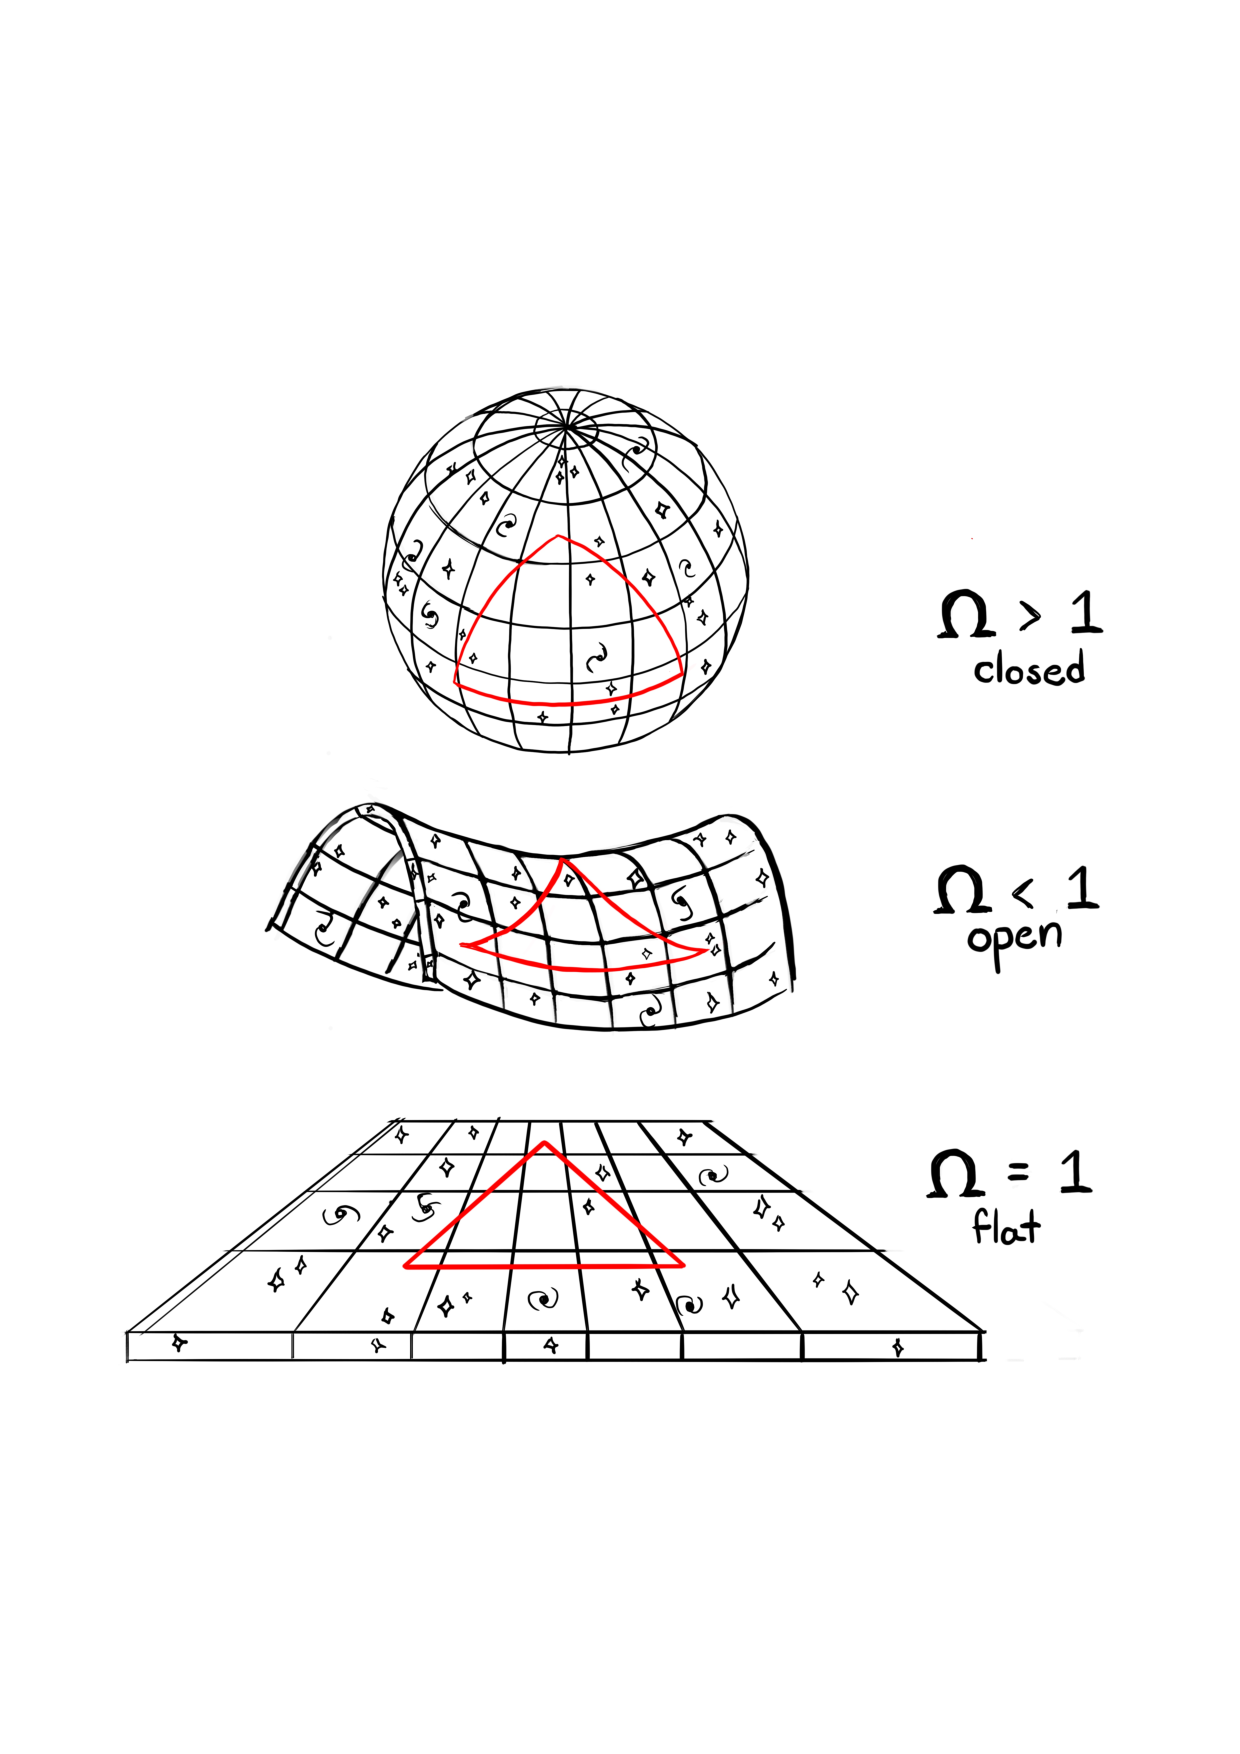
\includegraphics[width=\columnwidth]{Intro-FIGS/universeGeometry}
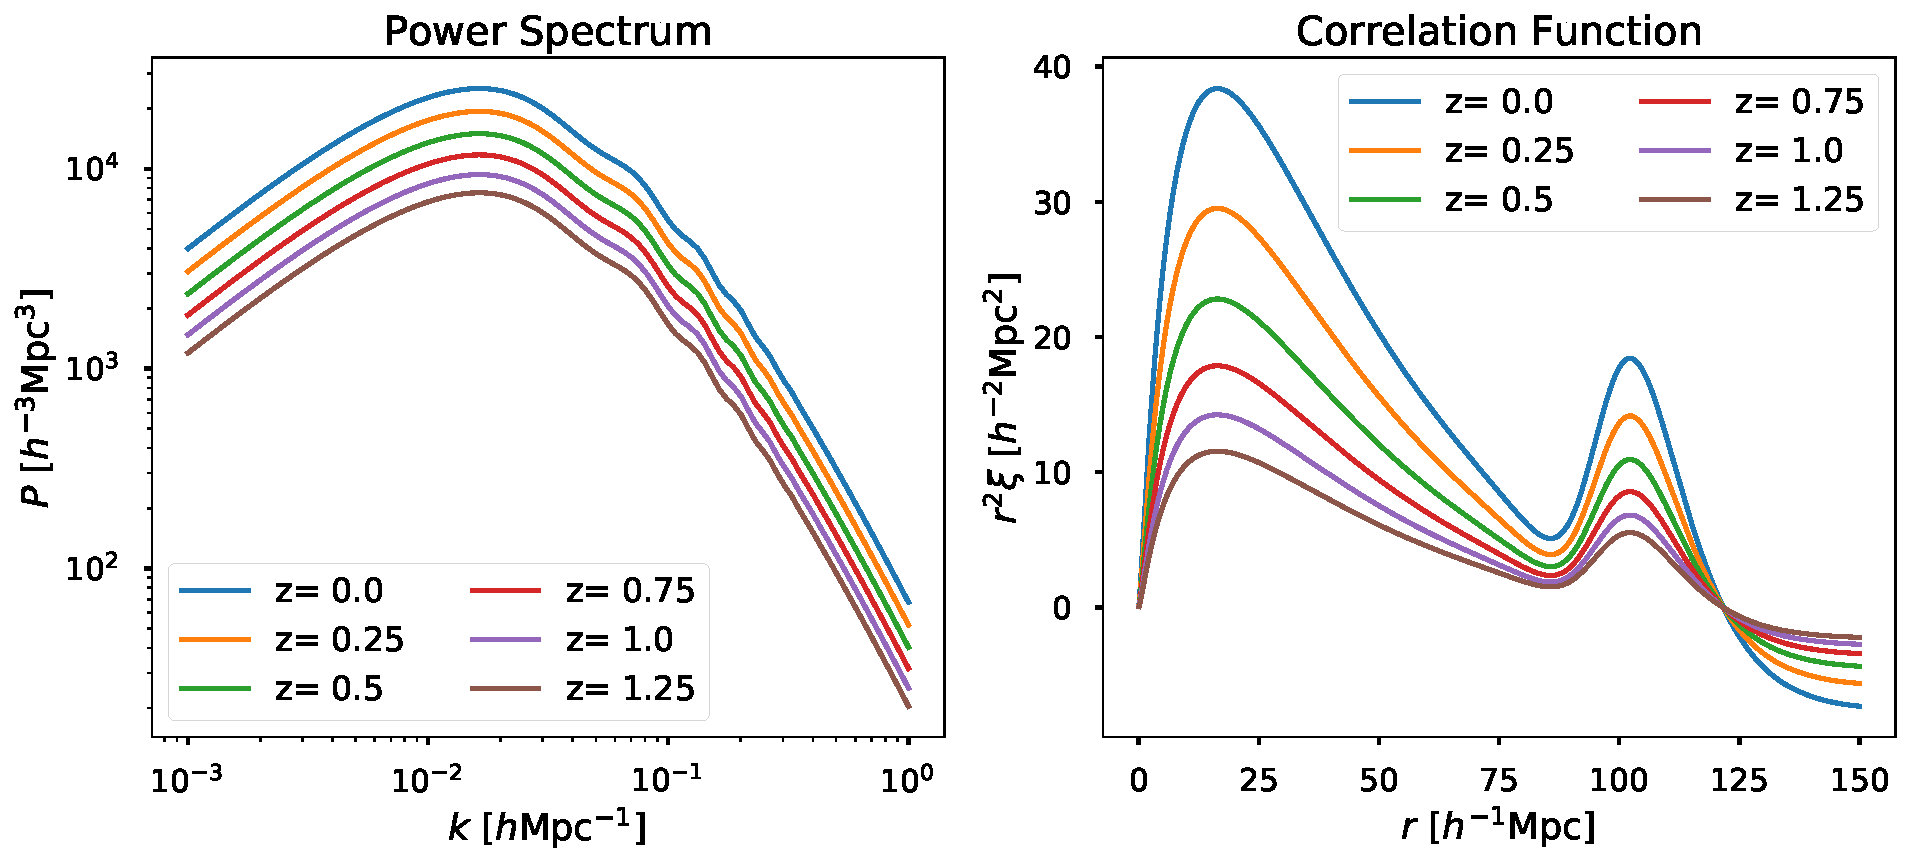
\includegraphics[width=\textwidth]{Intro-FIGS/Pk_Cf}
\caption[Power spectra and correlation functions calculated using the \class code.]{A series of power spectra and their Fourier counterparts, the correlation function, in different redshift ranges using a Planck 2015 fiducial cosmology \citep{PlanckResults2015} calculated using the \class code \citep{Class}. Note that the secondary peak in the correlation function (right) translates to wiggles in the power spectra (left), this is due to baryon acoustic oscillations in the primordial baryon-photon plasma.}
\label{fig:Pk_Cf}
\end{center}
\end{figure}

\qquad The growth factor determines the evolution of amplitude fluctuations in the Universe. A few approximations can be made in order to calculate this function and its redshift dependency; in a Newtonian approximation, for example, the growth function comes from solving the following differential equation \citep{schneider_2016}:
\EQ{}{
\ddot{D}(z) + \frac{2\dot{a}}{a}\dot{D}-4\pi G \bar{\rho}(z)D(z) = 0 \, ,
}
which, in terms of the scale factor, has the following solution at late times \citep{dods,schneider_2016}:

\EQ{}{
%D(a) = \frac{5\Omega_m}{2}\frac{H(a)}{H_0}\int_0^a \left( a' H(a')/H_0\right)^{-3}da'
D(a) = \frac{5\Omega_m}{2}\frac{H(a)}{H_0}\int_0^a \left[ \Omega_m/a' + \Omega_{\Lambda}a'^2 - (\Omega_m + \Omega_{\Lambda} -1 )\right]^{-3/2}da' \, ,
}
where a convention of $D(z=0)=1$ was used. The impact of $D(z)$ in the two-point statistics can be see in Figure \ref{fig:Pk_Cf} for a fiducial $\Lambda$CDM model.
%\subsubsection{Galaxy bias and non-linear scales:}

\qquad Dark matter, however, does not interact electromagnetically with baryonic matter which complicates any attempts to directly measure fluctuations in the underlying matter density field. Although no direct dark matter observations were made so far \citep{2017DarkMatterExpReview}, matter tends to cluster due to gravity, i. e. both dark and baryonic matter interact gravitationally. This causes baryonic matter, in the form of galaxies, clusters of galaxies, intergalactic gas, and more to act as a biased tracer of the underlying matter overdensity field, $\delta_g = b\delta$ \citep{2000-BensonBias,1999Ofer-Bias}. This bias can be represented as a function of several different aspects of galaxies: luminosity \citep{2000-BensonBias,2004PVP,2013Baugh-LumBias}, scale \citep{1999Ofer-Bias,2008ScaleBias,2008Hamann-ScaleBias,2018Simon-ScaleBias}, galaxy type \citep{2008Sanchez-Bias,2016AbramoSeccoLoureiro}, and redshift \citep{1994FKP,1998Heavens-Verde,2000-BensonBias}. The underlying physics in this process is that more massive halos will form more massive galaxies, which will have different star formation histories, affecting mainly these before-mentioned aspects. The work presented in the subsequent sections and chapters, considers bias simply to be a function of redshift as a first order approximation. Therefore, its impact on the power spectrum of galaxy distributions, $P_g(k)$, is 
\EQ{}{
P_g(k,k) = b^2(z)P(k,z) \, .
}

%%%%%%%%%%%%%%%%%%%%%%%%%%%%%%%%%%%%%%%%%%%%%%%%%%%%%%%%%%%
%				            BAO
%%%%%%%%%%%%%%%%%%%%%%%%%%%%%%%%%%%%%%%%%%%%%%%%%%%%%%%%%%%
\subsubsection{Baryon acoustic oscillations:}
The shape of both two-point statistics in Figure \ref{fig:Pk_Cf}, either in real or in Fourier space, raises attention to an interesting feature: the secondary peak in the correlation functions, manifested as wiggles in the power spectra. This peak is caused due to acoustic perturbation in the primordial baryon-photon plasma during radiation dominated era and are called baryon acoustic oscillations, or BAOs. Acoustic peaks were firstly observed in the CMB temperature angular power spectrum which raised the question if any similar features would appear in the large scale structure of galaxies. It was only in \cite{Einsenstein2005} that these BAO peaks were first measured using the correlation function of SDSS luminous red galaxies (LRGs).

%The tight coupling between baryons and photons in the primordial plasma during the radiation dominated era lead to what is called baryon acoustic oscillations, causing this peak to appear later on the statistical distribution of galaxies. These acoustic peaks were firstly observed in the CMB temperature angular power spectrum which raised the question if any consequences would appear in the large scale structure of galaxies. In \cite{Einsenstein2005}, this acoustic oscillations were first measured using the statistical distribution of SDSS luminous red galaxies (LRGs); the BAO peak was observed in the measured correlation function. 
\qquad The physical process behind the formation of BAO comes from the end of recombination era around $z \approx 1100$. The sound speed in the hot baryon-photon plasma decreased significantly and waves propagated due to the initial cosmological perturbations in this relativistic plasma. Baryons and photons were coupled both via Thompson scattering, gravitational attraction and radiation pressure; these couplings set up oscillations imprinting a characteristic length scale related to the oscillatory modes and the sound horizon at that epoch. Right after the period of recombination, the Universe goes through a period in which is non-ionised, `freezing' the baryonic oscillation scale while photons freely propagate. The density excess in the baryonic content of the Universe then interacts gravitationally with the non-coupled dark matter, later forming the distribution of galaxies with an imprinted acoustic peak.

\qquad Several fundamental conclusions, according to \cite{Einsenstein2005}, can be drawn from the BAO peak measurement. Initially, it provides very strong evidence that linear perturbation theory can be used in order to evolve the Einstein-Boltzmann equations (see Section \ref{Sec:Intro:LinTheory}) from redshift 1100 all the way to $z \approx 0$ -- at scales in which structure presents a linear behaviour. Another important conclusion comes from the interplay between dark and baryonic matter in order to form the BAO peak; a model with no dark matter present, purely baryonic, would not be able to reproduce the observed acoustic peak. Finally, the BAO peak provide cosmologists with a \textbf{standard ruler}, which can be measured over a wide range of redshifts, allowing us to probe the angular diameter distance along the line-of-sight together with the Hubble flow (Equation \ref{Eq:Intro:HubbleOmega1}). Currently, the most precise BAO measurements from galaxy surveys come from the BOSS Collaboration and are measured over a variety of methods -- see \citealt{2016BOSSCosmology} for a summary.

%%%%%%%%%%%%%%%%%%%%%%%%%%%%%%%%%%%%%%%%%%%%%%%%%%%%%%%%%%%
%		        	NON-LINEAR THEORY
%%%%%%%%%%%%%%%%%%%%%%%%%%%%%%%%%%%%%%%%%%%%%%%%%%%%%%%%%%%
\subsubsection{The non-linear power spectra:}
When dealing with smaller scales, at the order of clusters of galaxies, the linear theory approximation starts leading to imprecision in the power spectrum calculation. This is mostly due to the overdensity field's module tending to unity, which breaks down perturbation theory assumptions. Instead, different approaches are necessary. Computational calculation of non-linear overdensity amplitude fluctuations is usually performed with the use of N-body simulations with a wide range of cosmological parameters and fitting these to obtain power spectra predictions. The most used fitting is \texttt{HALOFIT} \citep{2003HaloFit,2012-Halofit,Bird2012} and its impact in the measured power spectra can be seen as an increase of power in smaller scales. Although a lot of collective effort has been put into perfecting these calculations over the years, as a rule of thump, the non-linear power spectrum is used to perform scale cuts in cosmological analyses\footnote{See Section \ref{Sec:CosmoAnal} in Chapter \ref{Chap:BOSS-Cosmo} for an example.} as even the latest advances on \texttt{HALOFIT} have around 5\% precision on scales up to $k\leq 1$ h/Mpc in $0\leq z \leq 10$ \citep{Takahashi2012,Bird2012}. 

%%%%%%%%%%%%%%%%%%%%%%%%%%%%%%%%%%%%%%%%%%%%%%%%%%%%%%%%%%%
%				WEAK LENSING
%%%%%%%%%%%%%%%%%%%%%%%%%%%%%%%%%%%%%%%%%%%%%%%%%%%%%%%%%%%
\subsection{Weak Lensing}
One of the earliest predictions from the General Theory of Relativity was that gravity should cause light to be distorted in specific ways, differently from what was predicted by Newtonian theory. Later, in 1919, by observing the background light of stars distorted by the Sun during an eclipse, this effect was confirmed in an expedition led by Sir Frank Dyson and Sir Arthur Eddington to Sobral in Brazil and the island of Principe in the African coast \citep{Dyson291}. Although some of the photosensitive plates from Eddignton's expedition to the island of Principe were compromised due to bad weather conditions, the ones taken in Sobral where more than sufficient to demonstrate that General Relativity passed its first ever test \citep{2007arXiv0709.0685K}.


\qquad Years after the eclipse, it is well known from General Relativity and observations that gravity causes light to bend like it does in the presence of lenses. One of the most impressive facts about this effect is that it allows for a reconstruction of dark matter's distribution even without the ability to properly observe it. As light is bend by matter, so it is by dark matter which deflects and distorts the shapes and sizes of background galaxies in relation to a massive foreground like a cluster. In first order, the lensing effects can be summarised by two phenomena: an isotropic dilatation called convergence, $\kappa$, and an anisotropic distortion called shear, $\gamma$. 

\qquad To understand these effects, one starts from an approximation of the lens equation -- which relates the true angle between an observer and an object, $\theta_{\text{src}}$, and the observed angle in the sky due to the bending of light, $\theta_{\text{obs}}$ \citep{dods}:

\EQ{}{
\theta_{\text{src},i} = A_{ij}\theta_{\text{obs},j}\, .
}
Here, the Jacobian matrix A can be related to convergence $\kappa$, the shear components $\gamma_1$ \& $\gamma_2$, and the Newtonian potential, $\Phi$, as

\EQ{}{
A_{ij} - \delta_{ij} = \left( \begin{matrix}
							- \kappa - \gamma_1 & -\gamma_2 \\
                             -\gamma_2  & -\kappa + \gamma_1
							\end{matrix} \right) 
                            = 2\int_0^{\chi}d\chi ' \Phi_{,ij}(\chi'\theta_{\text{obs}})\chi'\left(1-\frac{\chi'}{\chi}\right)\, ,
}
where $\chi$ is the comoving distance to the source and $\gamma^2 = \gamma_1^2 + \gamma_2^2$. In terms of observables, both shear and convergence can be estimated using a combination of measurements from galaxy ellipticities and mass surface projections. When observing the ellipticity of a galaxy, both shear and the intrinsic ellipticity are being measured. The intrinsic ellipticity is expected to be random \footnote{In first order. However, a lot of work has been done into understanding the role of the environment a galaxy is immerse in intrinsic alignments. See \cite{2015Kirk_IA} for a review.} and is averaged out when measured over enough background galaxies. 

\qquad Several galaxy surveys like DES \citep{2017arXiv170801530D}, KiDS \citep{2017MNRAS.465.1454H}, and CHFTLens \citep{2014CHFTLens} are focused in using weak lensing measurements for extracting cosmology, combining with galaxy clustering, producing mass maps of the dark matter field, between other applications. Chapter \ref{Chap:BPL} has a general discussion on measuring shear and polarisation power spectra from photometric galaxy surveys and CMB polarisation measurements as spin-2 fields. For a more general review on weak gravitational lensing methods, measurements, and theory please see \cite{2005astro.ph..9252S,2017SchpJ..1232440B}.

% \begin{itemize}
% \item Lensing potential
% \item Shear power spectrum
% \item Convergence
% \end{itemize}

%%%%%%%%%%%%%%%%%%%%%%%%%%%%%%%%%%%%%%%%%%%%%%%%%%%%%%%%%%%
%				BAYESIAN STATIS
%%%%%%%%%%%%%%%%%%%%%%%%%%%%%%%%%%%%%%%%%%%%%%%%%%%%%%%%%%%
\section{Bayesian Statistics Applied to Cosmology}\label{sec:intro:motivation}
Data analysis is at the core of the contemporary approach to cosmology. With the construction of bigger and more powerful telescopes, the amount of cosmological data present is increasing at an unprecedented rate. Such huge quantities of data can not be analyseD via `brute force' methods and compression of information is key, evoking the need of statistical analysis methods. Cosmology is unlike most sciences, the nature of our object of study is unique: the Universe. Cosmologists do not have the luxury of `turning the experiment's machine on and off again' in order to reproduce it; there is only one Universe implying that common statistical approaches (like a frequentist approaches) are not sufficient.

\qquad There are countless applications for Bayesian statistics in cosmology, ranging from photometric redshift estimations, cosmological parameter estimation, alternative ways to measure the power spectrum, and many more -- the last two are subjects of chapters in this work. In this section, I will focus on the application of Bayesian statistics to cosmological parameter estimation with a generic approach. Chapter \ref{Chap:BPL} presents an application to angular power spectra estimation.


\subsection{Bayes' Theorem and Marginalisation}
In cosmology, as in any other science, we want to be able to assert statements and hypothesis, assigning them `degrees of plausibility' which can be represented by `rules of probability' for consistent reasoning \citep{sivia2006data}. These can be represented, initially, by a very simple set of arguments:
\begin{enumerate}
\item Probabilities can be expressed by real numbers:
\EQ{}{
\Pr(\text{True}) = 1 \quad \text{as} \quad \Pr(\text{False}) = 0.
}
\item The probability of a certain hypothesis A increases as the probability of `not-A', or $\bar{A}$, decreases:
\EQ{Intro:Sum}{
\Pr(A|M) = 1 - \Pr(\bar{A}|M).
}
This is also known as the `sum rule' and M is the model or any underlying assumption made.
\item Two hypothesis can be related via a join hypothesis where the probability of A given B is expressed as:
\EQ{Intro:Product}{
\Pr(A,B|M) = \Pr(A|B,M)\Pr(B|M).
}
This expression is commonly known as `the product rule'.
\item The degrees of plausibility should be transitive in a sense that if A is more probable than B; B is more probable than C; than A is unquestionably more probable than C.

\item These plausibilities are independent of the order in which they are considered, depending only on the available data.
\end{enumerate}

%%%%%%%%%%%%%%%%%%%%%%%%%%%%%%%%%%%%%%%%%%%%%%%%%%%%%%%%%%%
%				DROP THE BAYES
%%%%%%%%%%%%%%%%%%%%%%%%%%%%%%%%%%%%%%%%%%%%%%%%%%%%%%%%%%%
\subsubsection{Baye's Theorem:}
\qquad In Bayesian statistics, the degree of plausibility is expressed in terms of a \textbf{posterior distribution}. This distribution relates the likelihood distribution to prior knowledge and the current evidence. Using both the sum and product rules, Bayes' theorem can be expressed as
\EQ{Intro:Bayes}{
\Pr(A|B,M) = \frac{\mathcal{L}(B|A, M)\Pi(A|M)}{\mathcal{Z}(B|M)}\, ,
}
where $\mathcal{L}(B|A, M)$ is the likelihood, the probability of the acquiring the data, B, given hypothesis A and model M; $\Pi(A|M)$ is the prior distribution, which is the probability of hypothesis A given prior knowledge on the model M; finally, $\mathcal{Z}(B|M)$, the normalisation factor, is called evidence and it is the probability of the data given the model only. The combination of these probability distribution functions (p.d.f.) leads to the posterior distribution, the plausibility of the hypothesis given the data and the underlying assumptions about the model. 

\qquad In other words, Bayes' theorem relates the probability over the veracity of a certain hypothesis given the data, to the probability that the data could have been measured in case where the hypothesis is true. This is the information encompassed into the likelihood function. However, it is the prior which differentiate Baysian statistics from the usual frequentist approach: it allows for previous knowledge to be incorporated into the assessment of the hypothesis's veracity. The prior distribution exhibit how much is known or unknown about the hypothesis' truth assertion before any data is analysed. 

%%%%%%%%%%%%%%%%%%%%%%%%%%%%%%%%%%%%%%%%%%%%%%%%%%%%%%%%%%%
%				MARGINALISATION
%%%%%%%%%%%%%%%%%%%%%%%%%%%%%%%%%%%%%%%%%%%%%%%%%%%%%%%%%%%
\subsubsection{Marginalisation and nuisance parameters:}
One of many advantages of Bayesian statistics is the possibility of dealing with parameters which need to be probed but are not of any particular interest, these are called `nuisance parameters'. In cosmology, nuisance parameters range from a instrumental calibration parameters to galaxy bias and redshift errors. Marginalisation is the key concept to deal properly with undesired parameters, and it is done by accounting for all possibilities related to the these parameter. Consider now a nuisance parameter, or hypothesis, B. One can account for it as a nuisance parameter by adding the probability of $\bar{B}$ in Equation \eqref{Eq:Intro:Product}:
\EQ{}{
\Pr(A,B|M) + \Pr(A,\bar{B}|M) = \left[ \Pr(B|A,M) + \Pr(\bar{B}|A,M)\right]\Pr(A|M),
}
where, with the use of Equation \eqref{Eq:Intro:Sum} the expression in brackets is unity in the above expression leading to
\EQ{}{
\Pr(A|M) = \Pr(A,B|M) + \Pr(A,\bar{B}|M)\, ,
}
meaning that the probability that the hypothesis A is true, independently of B being true, is the sum of probabilities of A and B being true plus A being true while B is not. Generally speaking, this expression translates to
\EQ{}{
\Pr(A|M) = \int_{-\infty}^{+\infty}\Pr(A,B|M)dB\, .
}

\qquad This method has a wide range of applications. An example of its power is that it allows for a much higher dimensional posterior, with a much simpler way to sample from, to be probed at the higher dimensional space and then marginalised over the dimensions of interest. This application such as this one is explored in Chapter \ref{Chap:BPL} for sampling from the joint distribution of spherical harmonics and angular power spectra, marginalising over the spherical harmonics coefficients, and obtaining a posterior for the power spectra.

%%%%%%%%%%%%%%%%%%%%%%%%%%%%%%%%%%%%%%%%%%%%%%%%%%%%%%%%%%%
%				DISFARÇAR AS EVIDENCIAS
%%%%%%%%%%%%%%%%%%%%%%%%%%%%%%%%%%%%%%%%%%%%%%%%%%%%%%%%%%%
\subsection{Evidence and Bayes Factor for Model Selection}
Although controversial in some aspects, the Bayesian evidence can be used to assess model selection. Treated as a normalisation factor for a long time, mostly due to the complications in calculating it, the evidence is an important piece of the Bayesian inventory and it is a natural by-product of nested sampling (discussed in more detail in Section \ref{Sec:Sampling}. Evidence calculations are more robust when their ratios are considered -- these are usually referred as `Bayes factors',
\begin{equation}
R_{A,B} = \frac{\mathcal{Z}(A|M)}{\mathcal{Z}(B|M)}
\label{Eq:Intro:BayesFactor}
\end{equation}
where here A and B can either be hypothesis or datasets. 

\qquad Another application for the Bayes factor is to assess consistency between combining two or more datasets. Considering three datasets, A, B, and C, the Bayes factor for combining these datasets given a model M is
\begin{equation}
R_{A,B,C} = \frac{\mathcal{Z}(A,B,C|M)}{\mathcal{Z}(A|M)\mathcal{Z}(B|M)\mathcal{Z}(C|M)}
\label{Eq:Intro:BayesFactor2}
\end{equation}
which, if much bigger than unity, favours the combination of datasets. 

\qquad As outlined in Chapter \ref{Chap:BOSS}, this method of model selection has received several criticism in the late years as values for the Bayes factor can have strong dependencies on the prior volume for each case. However, physically motivated priors should lead to reliable values for the Bayes factor, being then a reflection of the true consistency between datasets. Nonetheless, a plethora of new methods for model selection and dataset consistency assessment have been proposed by the community in the past few years. I have not explored this techniques in this work. For an investigation of a few of these new methods, please refer to \cite{2017CharnockTension,2018HuTension,2018FeeneyTension}.

%%%%%%%%%%%%%%%%%%%%%%%%%%%%%%%%%%%%%%%%%%%%%%%%%%%%%%%%%%%
%			    	PARAM_EST
%%%%%%%%%%%%%%%%%%%%%%%%%%%%%%%%%%%%%%%%%%%%%%%%%%%%%%%%%%%
\subsection{Parameter Estimation}\label{Sec:ParamEstSampling}
For a certain dataset, information regarding a given parameter's degree of plausibility is contained within the posterior distribution. A common way to summarise this information is via quoting best-fit points and confidence intervals (CI) or via a mean and a standard-deviation. The probability density of certain parameter's value is an evaluation of reliability that the true value is near the estimated one; this is usually given by the maximum of the posterior probability distribution function.

\qquad Consider $\{\theta_i\}$ to be the set of parameters in interest, $\vec{D}$ to be the data vector, M to be the model, and $\mathcal{P} = \Pr(\{\theta_i\}|\vec{D}, M)$ the posterior distribution. The set of best-fit estimates, $\Theta_{0,i}$, should be found near the maximum, i. e.
\EQ{}{
\left. \frac{\partial \mathcal{P}}{\partial \theta_i} \right\rvert_{\Theta_{0,i}} = 0
\quad \text{and} \quad
\left. \frac{\partial^2 \mathcal{P}}{\partial \theta_i^2} \right\rvert_{\Theta_{0,i}} < 0
}

\qquad For flat priors, the best estimates can be expressed mostly in terms of the log-likelihood, $\mathbb{L} = \ln \mathcal{L}(\vec{D}|\{\theta_i\},M)$, where 
\EQ{}{
\left. \frac{\partial \mathbb{L}}{\partial \theta_i} \right\rvert_{\Theta_{0,i}} = 0.
}
This log-likelihood can now be Taylor expanded into
\EQ{}{
\mathbb{L} = \mathbb{L}(\Theta_{0,i}) + \frac{1}{2} \sum^{N}_{i=1}\sum^{N}_{j=1} \left.\frac{\partial^2 \mathbb{L}}{\partial \theta_i \partial \theta_j} \right\rvert_{\Theta_{0,i}} (\theta_i - \Theta_{0,i}) (\theta_j - \Theta_{0,j}) + ...
}
Following, using a matrix notation in the Taylor expansion's first term, the likelihood takes a more familiar form,
\EQ{}{
\Pr(\bm{\theta}|\vec{D},M)\propto \exp\left[-\frac{1}{2}(\bm{\theta} - \mathbf{\Theta}_0)^T\bm{\nabla\nabla}\mathbb{L}(\mathbf{\Theta}_0)(\bm{\theta} - \mathbf{\Theta}_0)  \right] \, ,
}
a multivariate Gaussian distribution where the $N\times N$ matrix of second derivatives, $\bm{\nabla\nabla}\mathbb{L}(\mathbf{\Theta}_0)$, is related to Fisher information matrix -- and, consequently, the covariance matrix:
\EQ{}{
\mathcal{F}_{ij} = -(\bm{\nabla\nabla}\mathbb{L})_{ij} = \text{Cov}^{-1}_{ij}\, .
}
However, the Cram\'er-Rao theorem affirms that this equality only holds if the estimated best-fit value is truly at the maximum posterior for a multivariate Gaussian, otherwise $\text{Cov}_ij \geq \mathcal{F}^{-1}_{ij}$. Section \ref{Sec:LikelihoodsPriors} gets into the cosmological parameter estimation problem in more details.

%%%%%%%%%%%%%%%%%%%%%%%%%%%%%%%%%%%%%%%%%%%%%%%%%%%%%%%%%%%
%				MC MONTE-CARLO
%%%%%%%%%%%%%%%%%%%%%%%%%%%%%%%%%%%%%%%%%%%%%%%%%%%%%%%%%%%
\subsection{Monte-Carlo techniques for Bayesian inference}\label{Sec:Sampling}
Given the sizes of current data vectors in cosmology, a `brute force method' involving an N-dimensional grid interpolation of the posterior function in parameter space is completely out of question; an alternative method is necessary. Monte-Carlo techniques are a quick and reliable way to explore the posterior distribution's peaks and tails in a multi-dimensional space. Several different Monte-Carlo sampling techniques are widely used in cosmology where the main idea is to basically perform some sort of random walk in parameter space while probing the posterior distribution. 

\qquad Next, I will outline some examples of sampling techniques that are relevant for this work.

\subsubsection{Metropolis-Hastings:}
Metropolis-Hastings (MH) is one of the most common sampling techniques adopted by the cosmological community \citep{2002CosmoMC}. Even though I do not make use of this technique in this work, outlining it has a pedagogical importance as it sets the grounds for being one of the simplest sampling techniques to implement -- which also explains its popularity. In this algorithm, the walk in parameter space happens when the chain jumps from an initial position in parameter space, $\bm{\theta}_n$, to a next position, $\bm{\theta}_{n+1}$, with a transition probability function, $T(\bm{\theta}_n,\bm{\theta}_{n+1})$. This transition probability function ensures that the chain will have an asymptotic distribution that reflects the posterior's distribution. The selection of a new point is performed with the help of a proposal density distribution, $G(\bm{\theta}_n, \bm{\theta}_{n+1})$, which defines the new point based on the previous one. The new point is then accepted with a probability
\EQ{}{
\gamma(\bm{\theta}_n, \bm{\theta}_{n+1}) = \min \left\lbrace 1, \frac{\Pr(\bm{\theta}_{n+1}|\vec{D},M)G(\bm{\theta}_{n+1}, \bm{\theta}_{n})}{\Pr(\bm{\theta}_{n}|\vec{D},M)G(\bm{\theta}_n, \bm{\theta}_{n+1})} \right\rbrace \,
}
where here $T(\bm{\theta}_n,\bm{\theta}_{n+1}) = \gamma(\bm{\theta}_n, \bm{\theta}_{n+1})G(\bm{\theta}_n, \bm{\theta}_{n+1})$ guaranteeing that the sampled posterior is the Markov Chain equilibrium distribution:
\EQ{}{
\Pr(\bm{\theta}_{n+1}|\vec{D},M)T(\bm{\theta}_{n+1},\bm{\theta}_{n}) = \Pr(\bm{\theta}_{n}|\vec{D},M)T(\bm{\theta}_{n},\bm{\theta}_{n+1})\, .
}
This also ensures correlations between accepted points. The method converges purely with $n\rightarrow \infty$, but acceptable converse naturally occurs with a finite number of samples.

\subsubsection{Hamiltonian Monte-Carlo:}
Although MH is a very simple technique to implement, it has several limitations and it can be extremely time consuming if the number of dimensions increase. Hamiltonian Monte-Carlo (HMC) is a more sophisticated technique and it samples the posterior considering the evolution of Hamilton's equations -- which explains the name \citep{Taylor2008}. In this algorithm, consider the potential energy $\psi$ of a posterior distribution $\Pr(\bm{x})$ as the negative log-posterior,
\EQ{Intro:Pot_HMC}{
\psi(\bm{x}) = - \log\Pr(\bm{x}) \, .
}
In the expression above, $\bm{x}$ is the N-dimensional vector of parameters to be sampled, $x_i$. Each of the parameters are assigned to a momentum, $p_i$, and mass, $m_i$, such that the kinetic energy of this system of parameter-particles is defined as
\EQ{Intro:K_HMC}{
\phi(\bm{p}) = \sum_i^N \frac{p_i^2}{2m_i}\, .
}

\qquad Now, one can define the Hamiltonian of the system by using the potential and kinetic energies,
\EQ{}{
\mathcal{H}(\bm{x},\bm{p}) = \sum_i^N\frac{p_i^2}{2m_i} + \psi(\bm{x}) \, .
}
The main idea in this method is to sample from a distribution proportional to $\exp(-\mathcal{H})$ which can be expressed as
\EQ{Intro:HMC_ExpH}{
\exp(-\mathcal{H})\propto \Pr(\bm{x})\prod_i^N\exp\left(-\frac{1}{2}\frac{p_i^2}{m_i}\right)\, .
}

\qquad The distribution in Equation \eqref{Eq:Intro:HMC_ExpH} is now separated into a posterior distribution and a Gaussian containing the parameters' momenta. Now, one can marginalise over the momenta parameters while sampling at each new step -- as the momenta are nuisance parameters. To generate a new posterior sample, one starts by drawing a sample from the kinetic energy distribution -- an uncorrelated normal distribution with zero mean and a variance equal to the masses of the parameters. Starting with an initial point $(\bm{x}, \bm{p})$, this system can now be deterministically evolved using a fixed time parameter, $t$. A new point $(\bm{x}', \bm{p}')$ is found by evolving Hamilton's equations,
\EQ{Intro:HMC_Hamil}{
\frac{dx_i}{dt} & = \frac{\partial\mathcal{H}}{\partial p_i}\, ,\\
\frac{dp_i}{dt} & = \frac{\partial \mathcal{H}}{\partial x_i} = \frac{\partial \psi(\bm{x})}{\partial x_i} \, .
}
where a new point is accepted with probability $\gamma(\bm{x}, \bm{x}', \bm{p}, \bm{p}') = \min(1, exp(-\delta\mathcal{H}))$ and $\delta\mathcal{H}$ is the change in the Hamiltonian between the previous point and the proposed new one: $\delta\mathcal{H} = \mathcal{H}(\bm{x}, \bm{p}) - \mathcal{H}(\bm{x}', \bm{p}')$. If the trajectory conserves energy, than $\delta\mathcal{H} = 0$ and $\gamma =1$, so the point is accepted. 

\qquad More details in how to evolve Hamilton's equations for this algorithm and a extension to much higher dimensional problems are explored in Section \ref{Sec:BPL:GHS}.

\subsubsection{Nested Sampling:}
In the past few years, Nested Sampling's popularity is increasing considerably within the cosmological community. Its ability of sampling the posterior while probing the evidence allows for both parameter estimation and model selection simultaneously \citep{2004NestedSampling}. This algorithm --although containing different variations like \texttt{MultiNest} \citep{2009Multinest}, \texttt{PolyChord} \citep{2015PolyChord}, and \texttt{Pliny} \citep{PlinyRichardThesis} -- has a simple idea based in using a collection of $n_{\text{live}}$ objects $\bm{\theta}$, called `live-points', which were sampled from the prior distribution, but are constrained to be inside a certain value of the likelihood, $\mathcal{L}(\bm{\theta}) > \mathcal{L}^*$ \citep{sivia2006data}.

\qquad Firstly, the N-dimensional parameter prior space, $\Pi(\bm{\theta}|M)$, is transformed into a N-dimension unity cube. The live-points are randomly sampled within the prior volume subjected to a constrain related to $\mathcal{L}^*$:
\EQ{Intro:PriorVolume}{
\xi(\mathcal{L}^*) = \idotsint_{\mathcal{L}(\bm{\theta}) > \mathcal{L}^*} \Pi(\bm{\theta}|M)d\bm{\theta} \, .
}
All points are drawn within this space and their likelihoods are evaluated. The likelihood values are used to assess if a live-point is inside an iso-contour $\mathcal{L} = \mathcal{L}^*$, for a given $\mathcal{L}^*\geq 0$. The point with the lowest likelihood, $\mathcal{L}_{\min}$ is then identified and eliminated and new point is drawn inside the $\mathcal{L} = \mathcal{L}_{\min}$ contour. This process is repeated until the maximum likelihood value is found, always identifying likelihood iso-curvatures at each step until a final peak is identified.

\qquad Using this sampling technique, the evidence can be estimated simply by calculating
\EQ{}{
\mathcal{Z} = \int_0^1\mathcal{L}(\xi)d\xi
}
which becomes much simpler to evaluate in this algorithm as one does not need now to evaluate a N-dimensional integral, which, in this case is simply a Riemann sum of the weights.

%%%%%%%%%%%%%%%%%%%%%%%%%%%%%%%%%%%%%%%%%%%%%%%%%%%%%%%%%%%
%			            SURVEYS
%%%%%%%%%%%%%%%%%%%%%%%%%%%%%%%%%%%%%%%%%%%%%%%%%%%%%%%%%%%
\section{State-of-the-art Cosmological Probes}\label{sec:intro:probes}
In this section I will outline some of the state-of-the-art past, current, and future surveys used in the following chapters -- either to extract cosmological information from, or to forecast future cosmological endeavours.

\subsection{Planck Satellite}
\begin{figure}
\begin{center}
%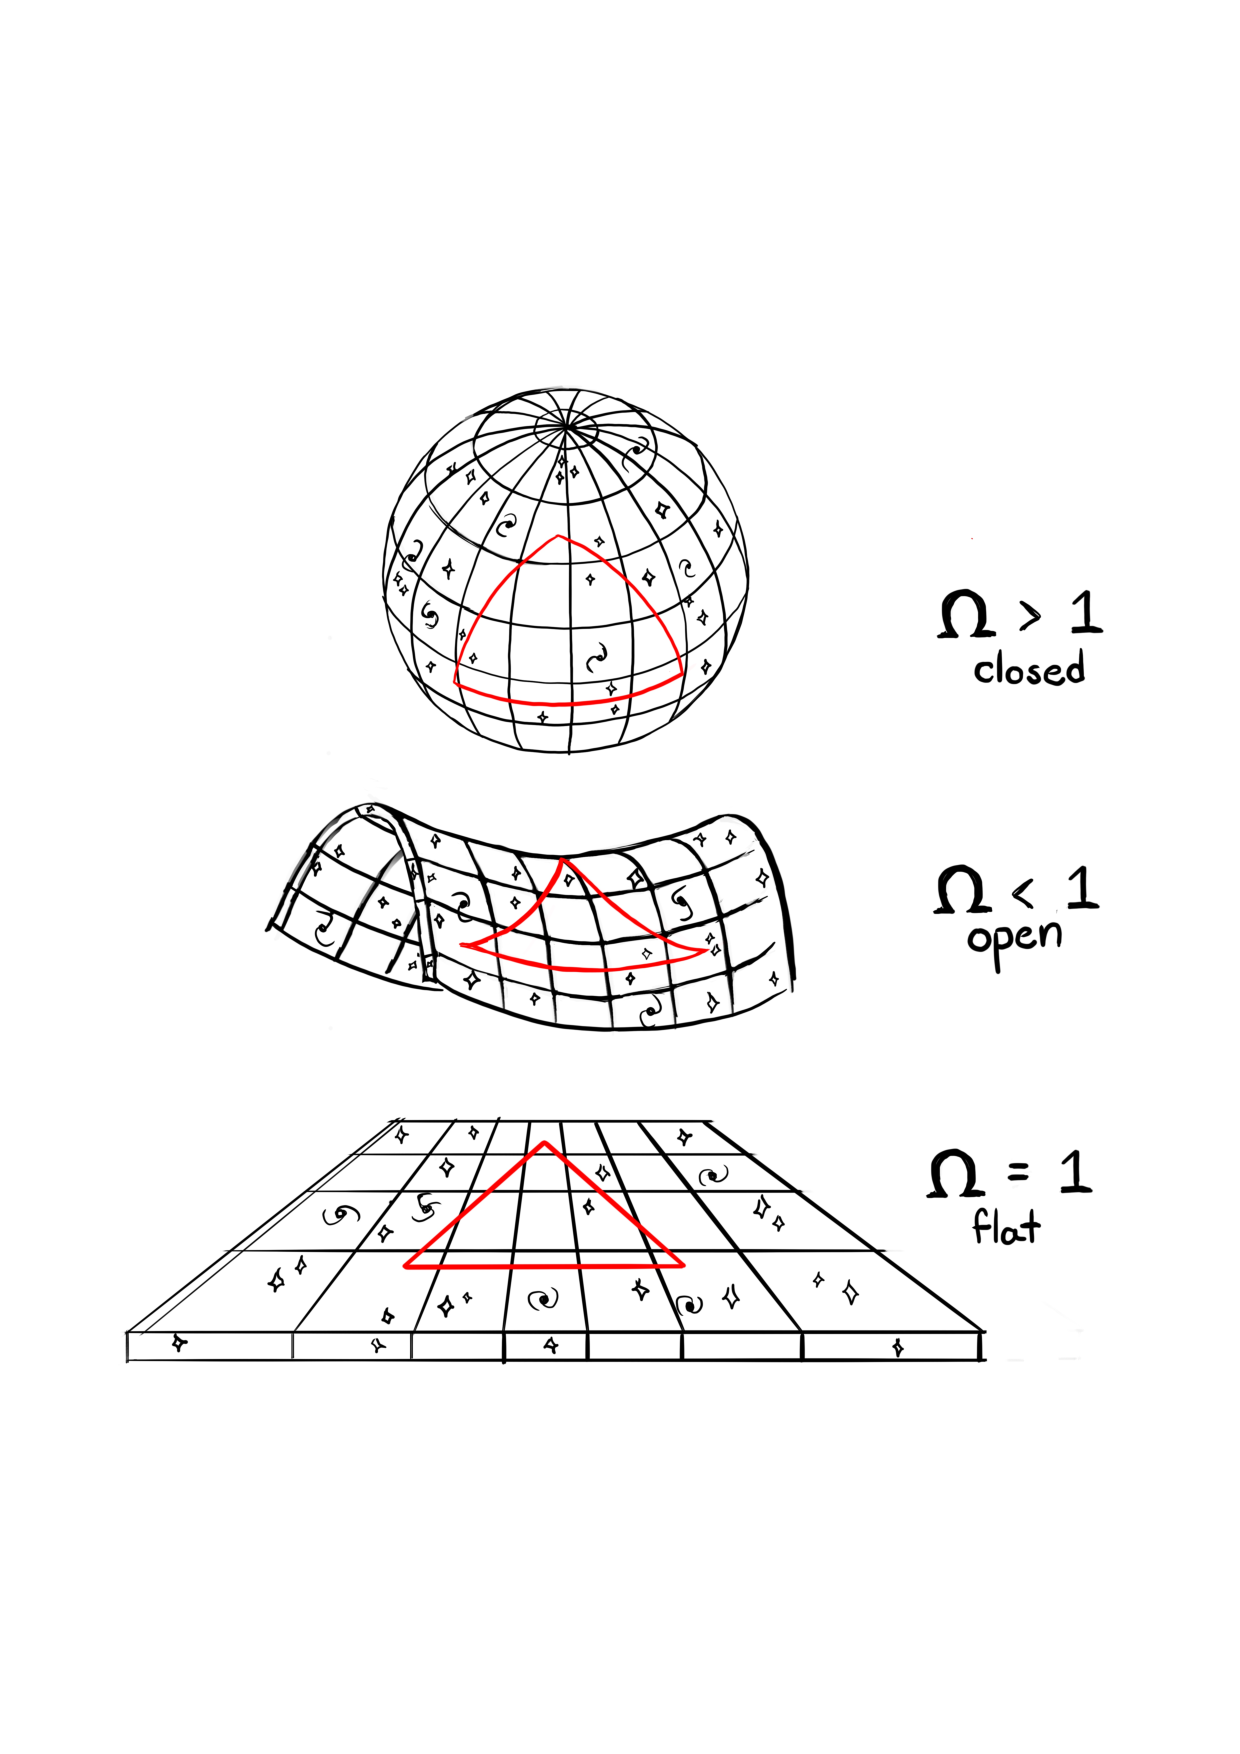
\includegraphics[width=\columnwidth]{Intro-FIGS/universeGeometry}
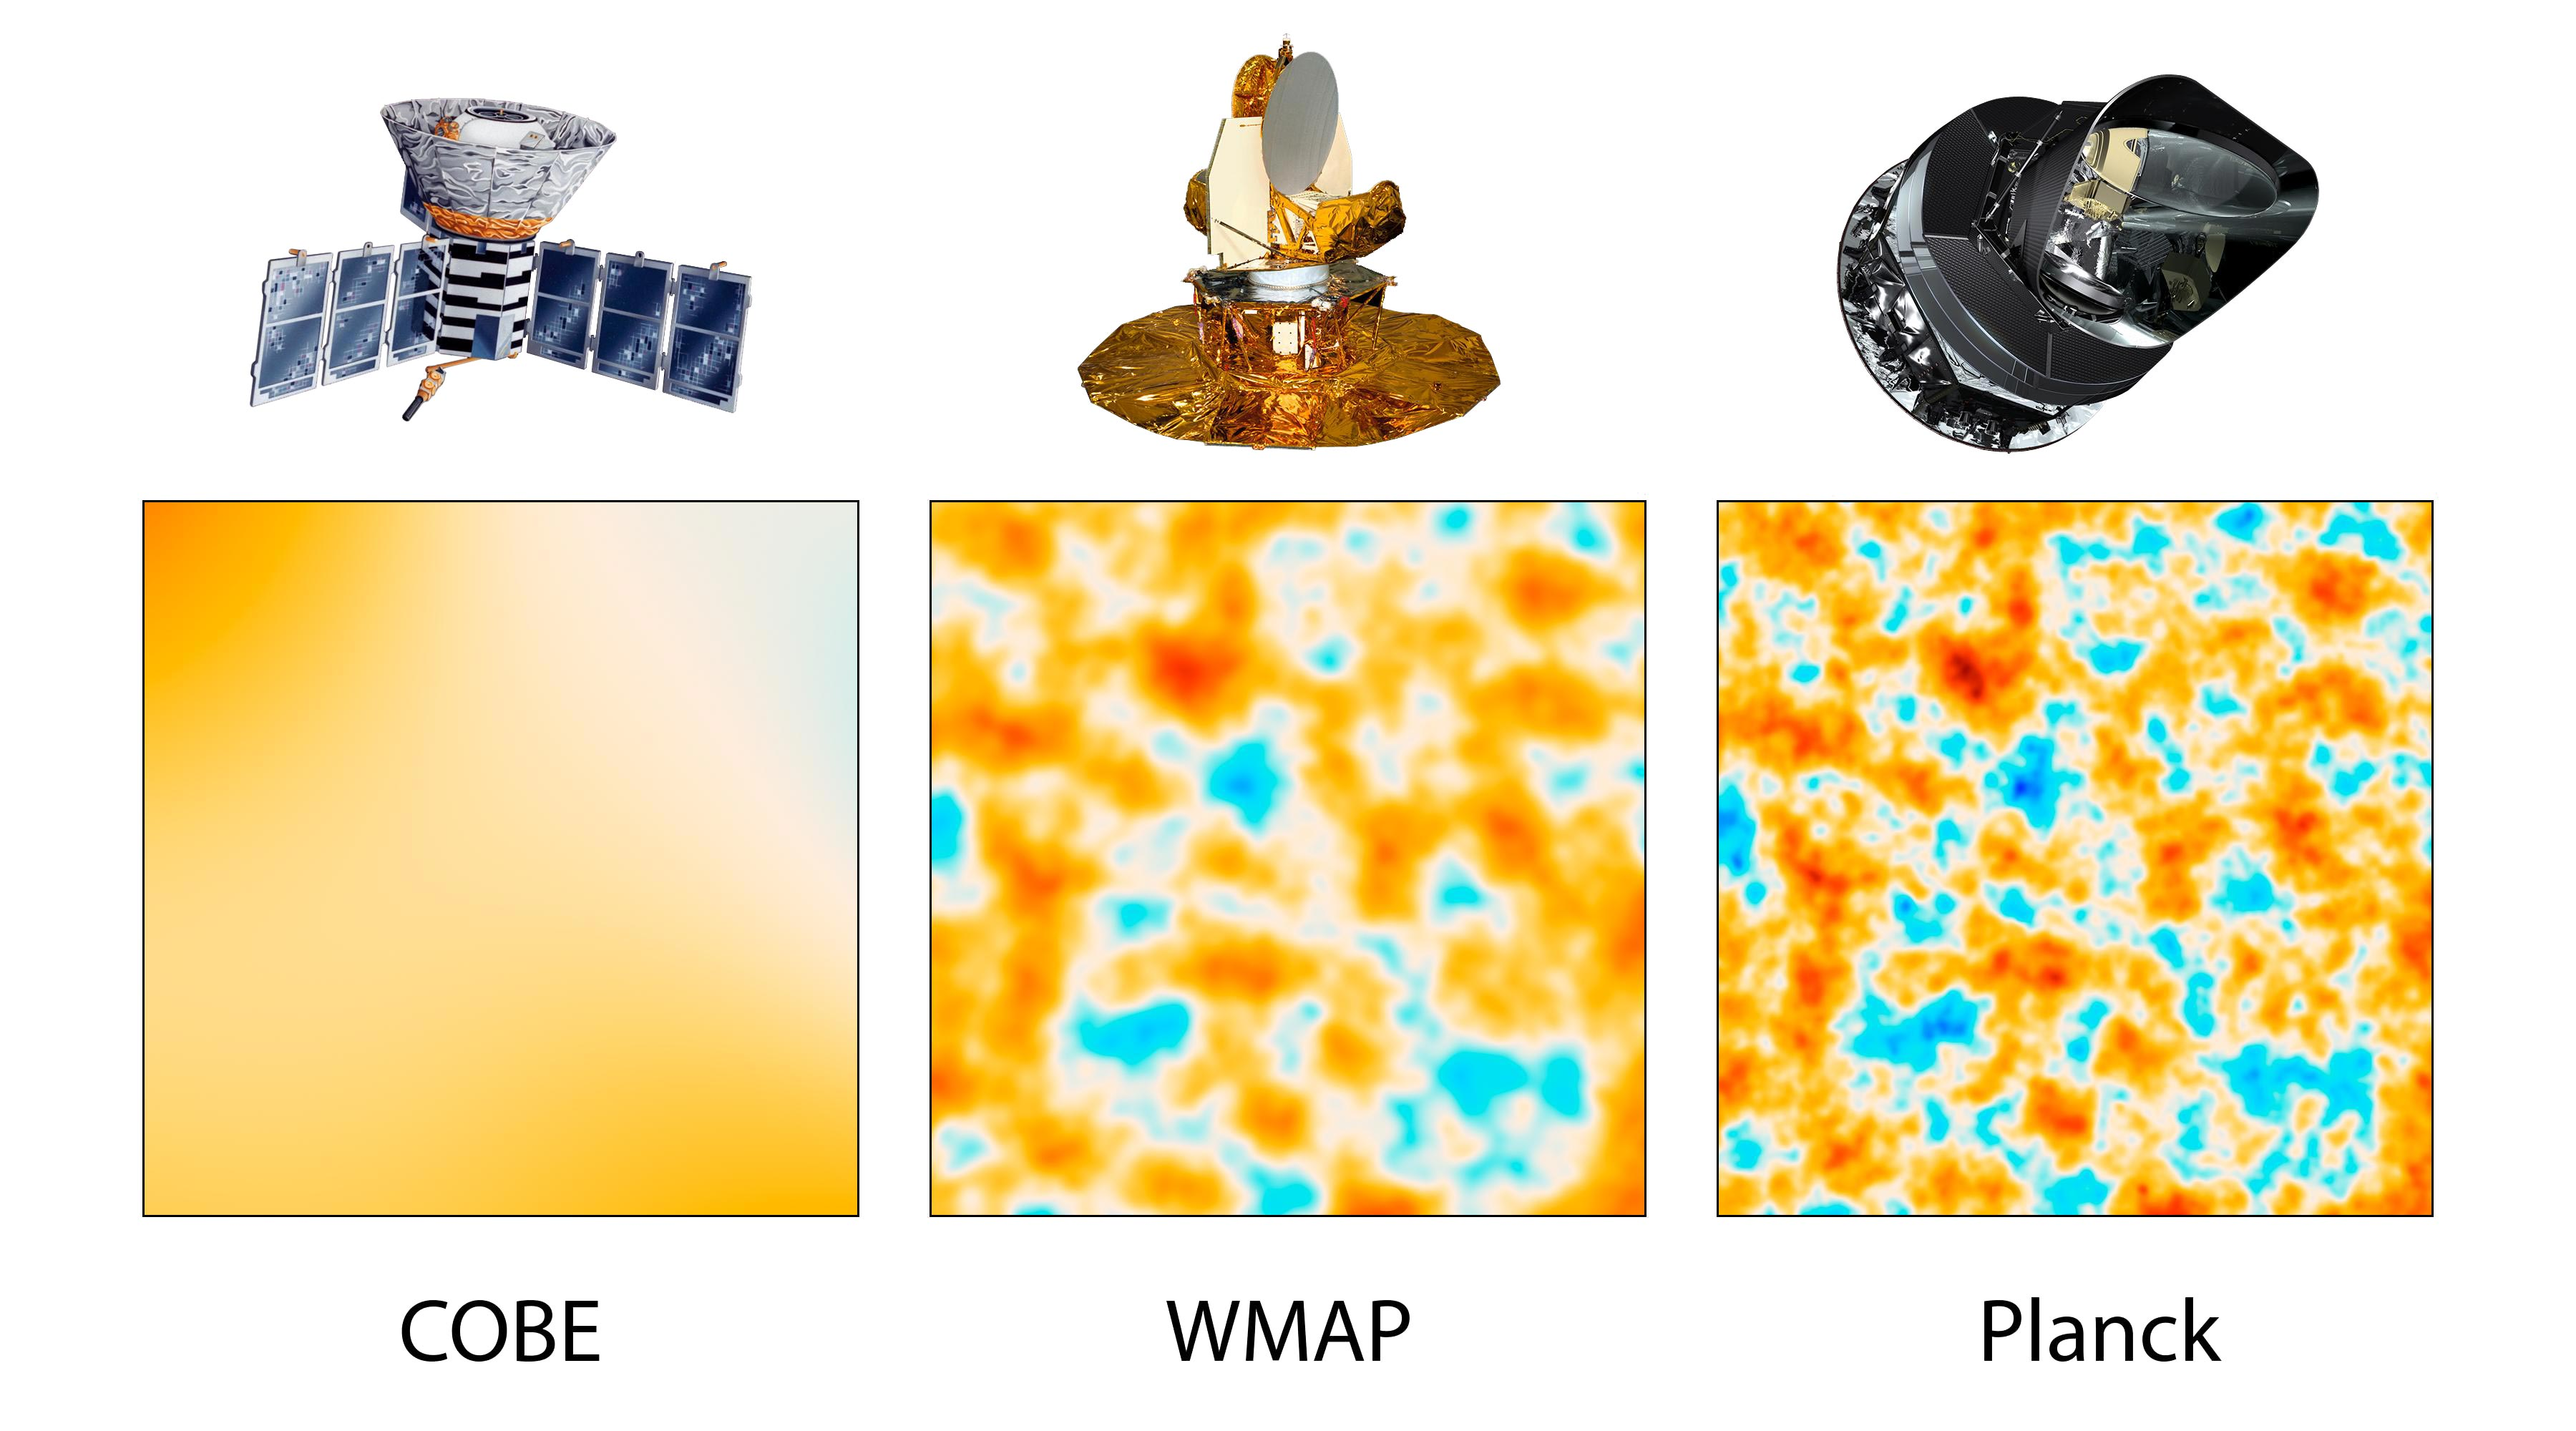
\includegraphics[width=\textwidth]{Intro-FIGS/planck_wmap_cobe.jpg}
\caption[A comparison between three generations of space CMB experiments. Image credit: NASA/JPL-Caltech/ESA.]{A comparison between the resolutions of COBE \citep{COBE}, WMAP \citep{WMAP_MapsResults}, and Planck \citep{planck2013} and the respective cosmic microwave background temperature maps. Panels show the same 10 deg$^2$ patch of the sky where the Planck resolution is around $5'$ whereas COBE's resolution is $7^o$ and WMAP's resolution is $20'$. Image credit: NASA/JPL-Caltech/ESA.}
\label{fig:PlanckWMAPCOBE}
\end{center}
\end{figure}
The Planck Satellite \citep{planck2013} is an European Space Agency telescope, situated at the L2 Lagrangian point of the Earth-Sun's system, aimed to make observations of the Cosmic Microwave Background, the first light of the Universe as it became transparent to electromagnetic radiation at the end of recombination era around 13.3 billion years ago. The Planck Satellite is a part of what is called a `Stage 3' CMB experiment and it took data between 2009 and 2013. Previous space-based CMB experiments are the Wilkinson Microwave Anisotropy Prope (WMAP, \citealt{WMAP_MapsResults}) working between 2001 and 2010, and the Cosmic Background Explorer (COBE, \citealt{COBE}) working between 1989 and 1993. Differently from its predecessors, the Planck Satellite contained very sensitive detectors, capable of measuring the polarisation of CMB photons with great accuracy and the temperature spectrum with impressive resolution. Figure \ref{fig:PlanckWMAPCOBE} shows a comparison between the three probes' resolutions in the same 10 deg$^2$ patch of the sky.


\qquad With impressively good resolution for temperature and polarisation measurements, having taken data in nine different frequencies, the Planck Collaboration released to date three cosmological parameter estimation results using temperature and polarisation auto- and cross-power spectrum, CMB lensing and low-mode polarisation \citep{planck2013,PlanckCosmology2016,2018PlanckCosmology}. The latest results were released in 2018 and are presented in \cite{2018PlanckCosmology} \footnote{The cosmological likelihood codes for the 2018 results are not available to date.} constituting one of the most precise and reliable cosmological measurements to date with percent level constraints in early Universe cosmological parameters like the primordial power spectrum amplitude, $A_s$; the scalar spectral index, $n_s$; the reionisation's optical depth, $\tau$, and more. Details on how Planck's data are used in this work are presented in Section \ref{Sec:ExternalData}.

% \begin{itemize}
% \item outline the survey
% \item what Planck measures
% \item what is considered in this work about it
% \item temperature, polarisation, lensing
% \item description of their cosmological findings
% \end{itemize}

\subsection{Baryon Oscillation Spectroscopic Survey}
As a part of the Sloan Digital Sky Survey (SDSS) Phase-III, the Baryon Oscillation Spectroscopic Survey (BOSS, \citealt{2013BOSS-Whitepaper}) is currently the largest galaxy redshift survey and it is the main dataset used in Chapters \ref{Chap:BOSS} and \ref{Chap:Neutrinos}. The main purpose of BOSS is to perform a spectroscopic follow-up of SDSS photometric luminous red galaxies and quasars using a multiple-object spectrograph. The survey ran between 2008 and 2014 and obtained spectra for more than 1.5 million galaxies up to $z\approx 0.8$ \citep{BOSSCatalogue2016} and 160,000 quasars between $2.2 < z < 3$ using the Lyman-$\alpha$ spectra \citep{2013LyAlphaBOSS}.

\qquad The main objective of BOSS Collaboration was to measure and obtain cosmological parameters from the BAO scale across a variety of redshifts and methods\footnote{\citep{2017RossBOSS,2017BeutlerBOSS,2017Beutler2BOSS,2017SatpathyBOSS,2017SanchezBOSS,2017GriebBOSS,2017SalazarBOSSwTheta,2017WangBOSS,2017ZhaoBOSS}}. Using LRGs, the Collaboration obtained angular diameter distance and Hubble flow measurements with $\sim 2\%$ precision for intermediate redshifts, $0.3 < z < 0.55$, with a similar precision achieved using Ly-$\alpha$ quasars \citep{2013LyAlphaBOSS}. A compilation of BOSS Collaboration results for the galaxy sample can be found in \cite{2016BOSSCosmology} together with their consensus results for the last BOSS data release, DR12. A much more detailed discussion of the BOSS LSS galaxy sample, including target selection criteria, angular selection functions, redshift distribution, and more can be found in Section \ref{Sec:Data}.

% \begin{itemize}
% \item SDSS-III description
% \item main goal and outline
% \item BOSS BAO description
% \item the consensus cosmology
% \end{itemize}

% \subsection{Dark Energy Survey}
% \RED{I don't actually use DES, do I?}
% \begin{itemize}
% \item DES description
% \item 3x2pts statistics analysis
% \item Talk about their Y1 results
% \end{itemize}

\subsection{Euclid Satellite}
The Euclid Satellite is a future European Space Agency mission which will perform a 6 year long near-infrared and visual observations over 15,000 deg$^2$ for its wide angle survey, and a 40 deg$^2$ deep survey \citep{2011EuclidRedPaper}. The satellite will observe the sky in three different ways: photometric visible imaging in R+I+Z bands (550-900 nm) and near-infrared imaging in three different bands -- Y (920 - 1146 nm), J (1146 - 1372 nm), and H (1372 - 2000 nm) --, and a near-infrared slit-less spectroscopy (1100-2000 nm) over all the survey area. The visual imaging instrument has $0.1 ''$ resolution, while both the NIR instruments have an angular resolution of $0.3''$.

\qquad Euclid's primary science goal is to probe the expansion and structure formation history of the Universe up to redshift $z\sim 2$. Combining state-of-the-art imaging and slit-less spectroscopy makes Euclid the ultimate cross-correlations machine. Euclid will be able to combine large scale structure of galaxies, with outstanding photometric and spectroscopic redshift precision, $\sigma^{\text{photo}}_z/(1+z) < 0.05$ and  $\sigma^{\text{spec}}_z/(1+z)< 0.001$, respectively. Galaxy shape measurements for cosmic shear will have an equally impressive precision \citep{2016SartorisEuclid,2016SellentinWLEuclid}. Combining these probes in a concise framework is key to achieve the necessary precision to measure Euclid science goal's key cosmological parameters: the evolution of dark energy's equation-of-state, $w(z)$; the growth factor in a framework of modified gravity, $\gamma$; the sum of neutrino masses, $\sum m_{\nu}$, and their hierarchy; and the non-Gaussianity parameter, $f_{NL}$, related to inflationary models \citep{2011EuclidRedPaper}.

\subsection{Supernovae Type Ia Compilations}
\begin{figure}
\begin{center}
%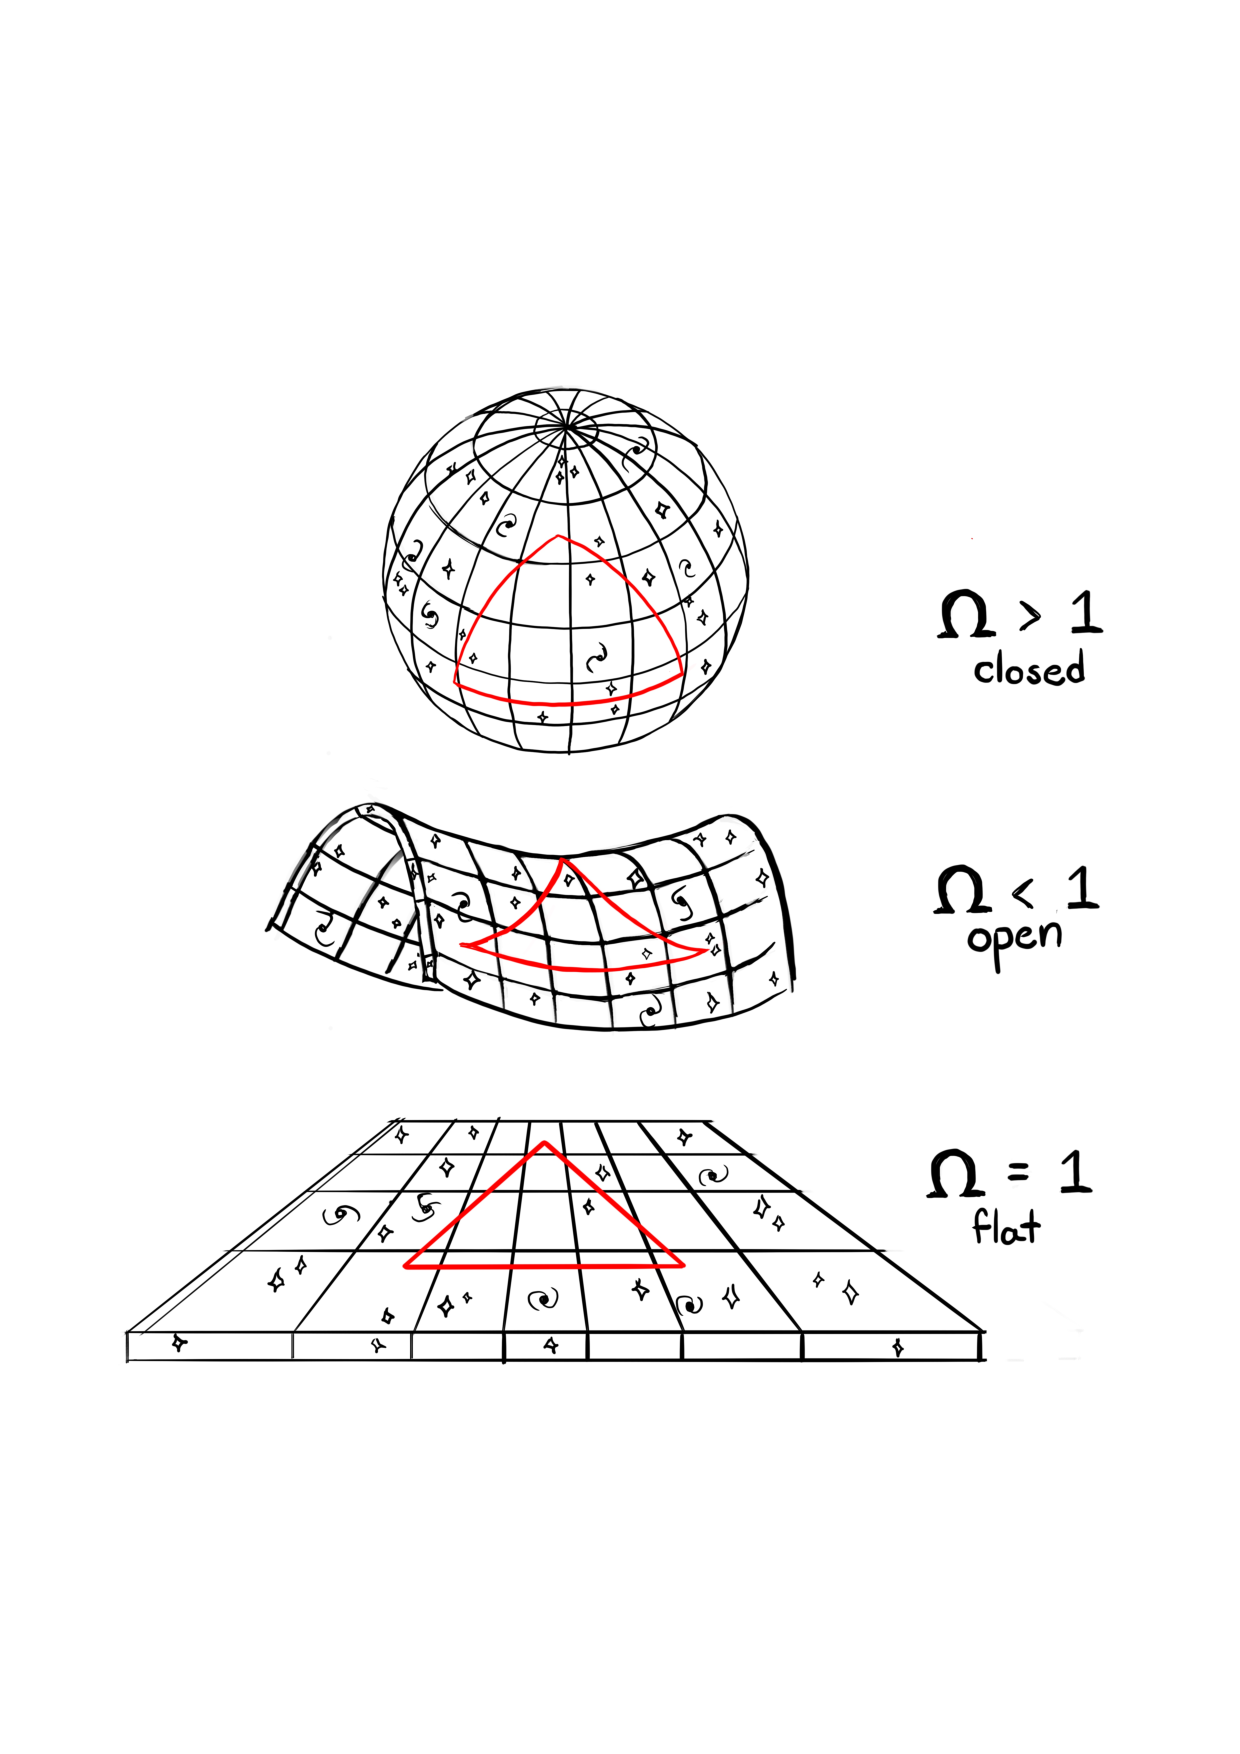
\includegraphics[width=\columnwidth]{Intro-FIGS/universeGeometry}
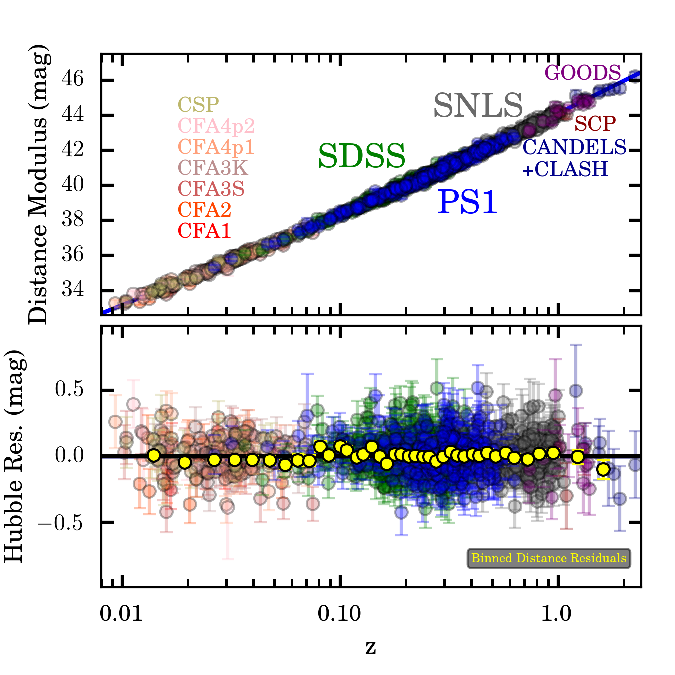
\includegraphics[width=\textwidth]{Intro-FIGS/hubble.pdf}
\caption[Hubble Diagram for the Pantheon Sample. Image credit: \cite{2018Pantheon}.]{Hubble Diagram for the Pantheon Sample. The \textit{top panel} shows the distance module as a function of redshift while the \textit{bottom panel} shows the residuals for the best-fit $\Lambda$CDM cosmology, $\Delta \mu \equiv \mu - \mu_{\text{best-fit}}$. Note that the Pantheon Sample contains the JLA sample as it can be seen as an updated version of it, including some new SNe Ia from the Pan-STARRS Survey \citep{2016-PanStarrs}. Image credit: \cite{2018Pantheon}.}
\label{fig:Pantheon}
\end{center}
\end{figure}
Supernovae Type Ia (SNe Ia) light-curve analysis compilation are crucial to cosmological data analysis; they were the first tools used to confirm that our Universe is going through a phase of accelerated expansion \citep{1998Riess,1999Perlmutter}. After being photometrically detected by differential imaging, spectroscopically confirmed SNe Ia have accurate redshift measurements and can be used as standardisable candles. This analysis is done via comparing the observed, $m_{\text{obs}}$, and the corrected magnitude, $M$, of a high redshift SNe Ia sample. One can then infer which set of cosmological parameters best-fits the so-called `distance modulus', defined as \citep{2007Salt-2,JLAdata}
\begin{equation}
    \mu = m_{\text{obs}}^* - (M_B + \alpha x_1 - \beta c)
\end{equation}
where $m_{\text{obs}}^*$ is, usually, the observed peak magnitude in the $B$-band, while the other parameters, $M_B, \alpha$, and $\beta$ are nuisance parameters. Some of these parameters, such as $M_B$ and $\beta$ are known to have a dependency on the host galaxy environment \citep{2011Sullivan}. The distance modulus can be compared with theoretical predictions using the following expression:
\begin{equation}
    \mu_{\text{th}}(z) = \lo(d_L(z)/10\, \text{pc})\, ,
\end{equation}
where the distance, $d_L$, is defined as 
\begin{equation}
    d_L(z) = \frac{1}{H_0}\lim_{\Omega_k' \rightarrow \Omega_k}\frac{(1+z)}{\sqrt{\Omega_k'}}\sinh\left( \sqrt{\Omega_k'}\int_0^z\frac{dz'}{E(z')}\right)
\end{equation}
with $E(z)$ defined as in Equation \eqref{Eq:Intro:HubbleOmega2}.

\qquad Throughout this work I make use of two Supernovae Type Ia (SNe Ia) light-curve analysis compilation. The first sample, used in Chapter \ref{Chap:BOSS}, is the Joint Light-curve Analysis (JLA) compilation \citep{JLAdata}; it contains spectroscopically confirmed SNe Ia from low redshift surveys, HST, SNLS \citep[all three presented in ]{2011Conley}, and SDSS-II \citep{2018Sako} -- with a total of 740 SNe Ia. The second sample, used in Chapter \ref{Chap:Neutrinos}, is the Pantheon compilation \citep{2018Pantheon}. It extends the JLA sample with the addition of spectroscopically confirmed SNe Ia from the Pan-STARRS Survey, with a total of 1048 SNe Ia with redshifts ranging from $0.01 < z < 2.3$. Details of the Hubble diagram for the Pantheon SNe Ia compilation and, consequently, from the JLA compilation can be found in Figure \ref{fig:Pantheon}.

\subsection{Big Bang Nucleosynthesis}
Big Bang Nucleosynthesis (BBN) is a very broad and extensive area of cosmology, here I present a very brief review of the relevant areas of this field for the present work. A complete review can be found in \cite{2007Steingman-BBN} and \cite{2016Particle-Review}.

\qquad Around the first twenty minutes of the Universe, the production of most of what it is considered to be `light elements' took place. These are $^3$He,$^4$He, D, and $^7$Li \citep{2007Steingman-BBN}. Th abundances of such primordial elements provide us with information about the conditions of the Universe at very early stages, the very first minutes after what it is believed to be a `Big Bang'. At sufficiently high temperatures and densities for the primordial plasma, both protons and neutrons will fuse to form atomic nuclei. The main baryonic reactions at the very early Universe maintain chemical equilibrium, these are \citep{2016Particle-Review}:
\begin{align}
    p + e^- & \longleftrightarrow n + \nu \, , \label{Eq:proton1}\\
    p + \bar{\nu} & \longleftrightarrow n + e^+ \, ,\label{Eq:proton2}\\
    n & \rightarrow p + e^- + \bar{\nu}\, . \label{Eq:neutronDecay}
\end{align}

\qquad The reactions shown in Equations \eqref{Eq:proton1} and \eqref{Eq:proton2} are related to keeping the proton-to-neutron equilibrium ratio, while Equation \eqref{Eq:neutronDecay} is the free neutron decay with a time-scale of $\tau_n \approx 880$s. The ratio of the number of protons, $n_p$, to the number of neutrons, $n_n$, can be expressed via the Boltzmann factor in tems of the mass difference between the two particles, $\Delta m_{n,p} = m_n - m_p \approx 1.293$ MeV \citep{2015NeutronProtonRatio}:
\begin{equation}
    \frac{n_n}{n_p} = \exp\left[ - \frac{\Delta m_{n,p}}{k_b T}\right]\, .
    \label{Eq:BoltzFactorNeutronProton}
\end{equation}
As soon as the neutrinos freeze-out, this ratio is kept almost constant at $n_n/n_p \approx 1/3$. After this period of decoupling, this equilibrium between protons and neutrons is broken and no longer described by the Boltzmann factor in Equation \eqref{Eq:BoltzFactorNeutronProton}, the changes in this ratio are then governed to the decay of free neutrons on the above-mentioned time-scale, $\tau_n$. For neutrons to `survive' throughout the history of the Universe, these need to be found in the nuclei of atoms \citep{2007Steingman-BBN}.

\subsubsection{Deuterium and Helium abundances:}

\begin{figure}
\begin{center}
%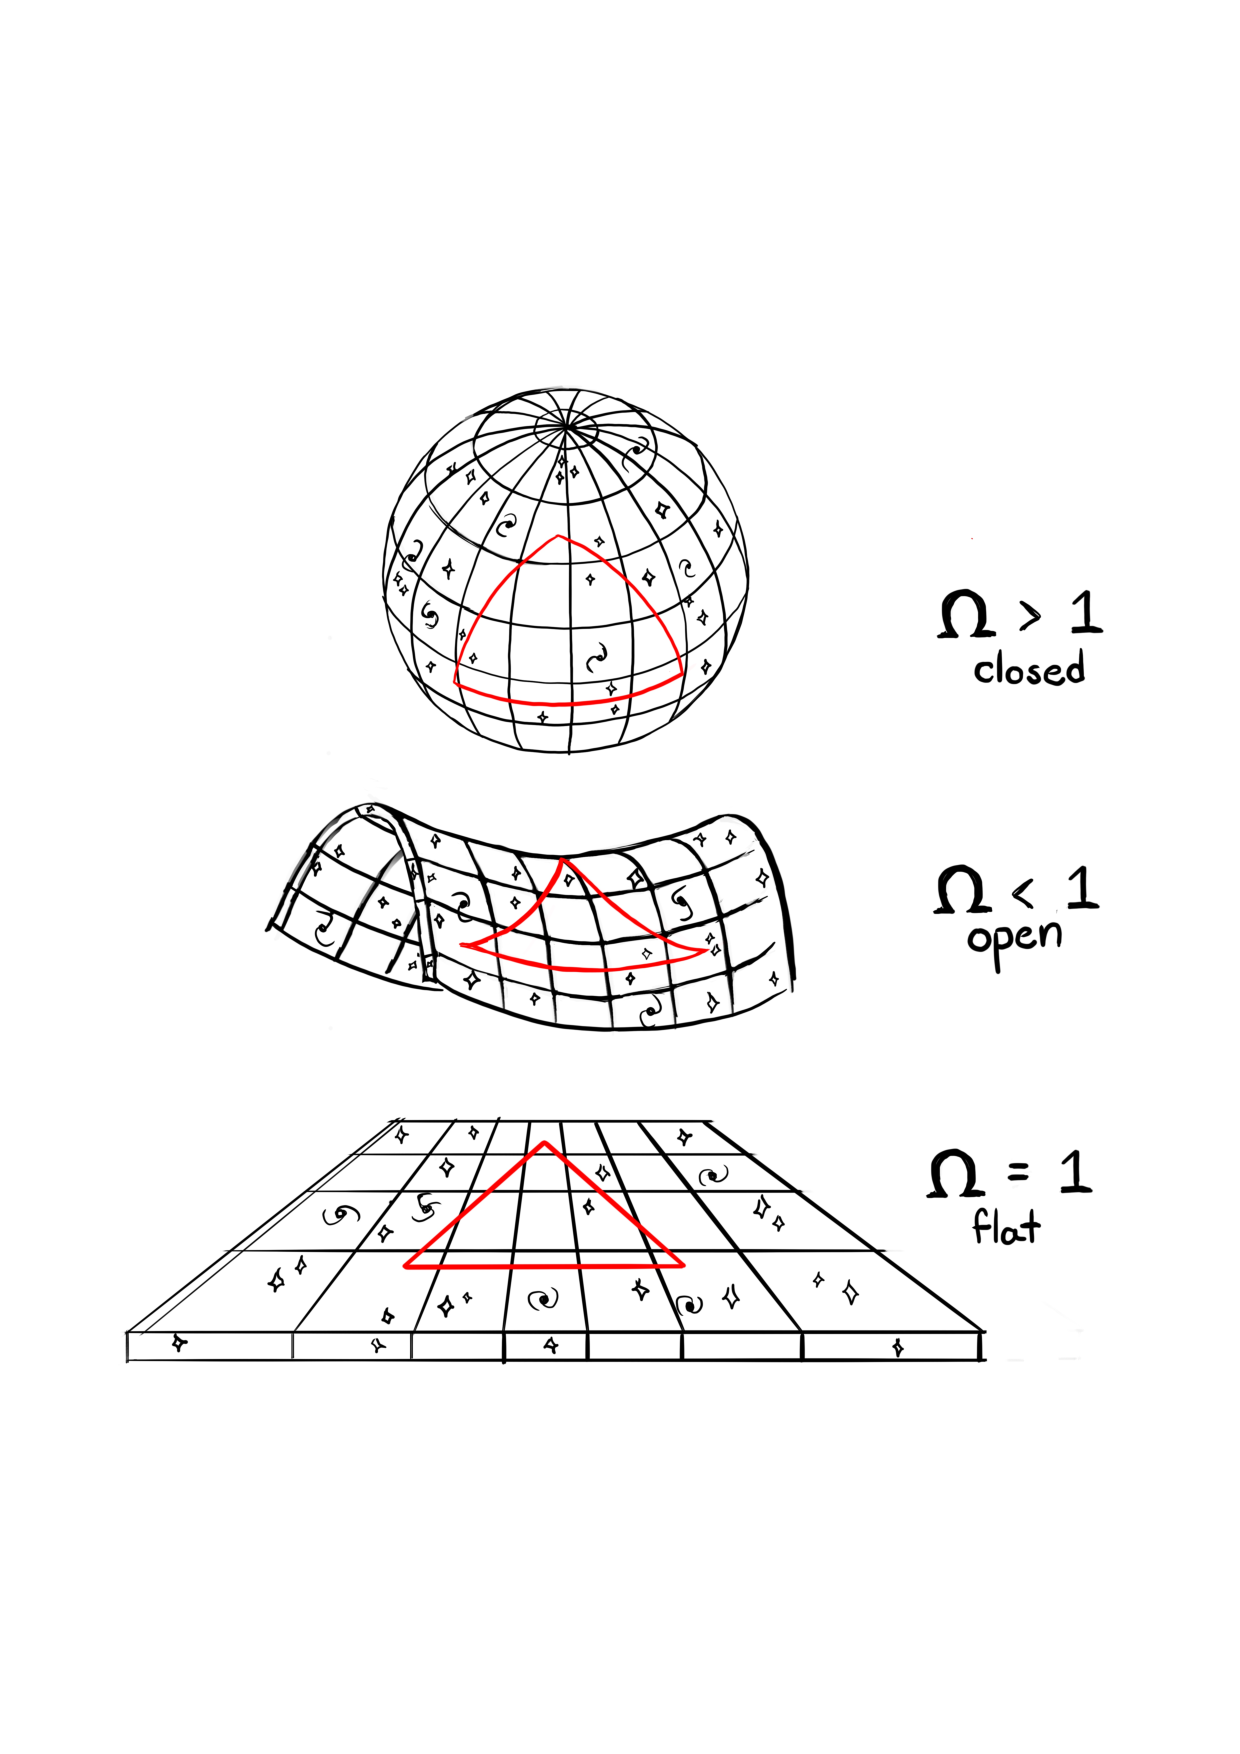
\includegraphics[width=\columnwidth]{Intro-FIGS/universeGeometry}
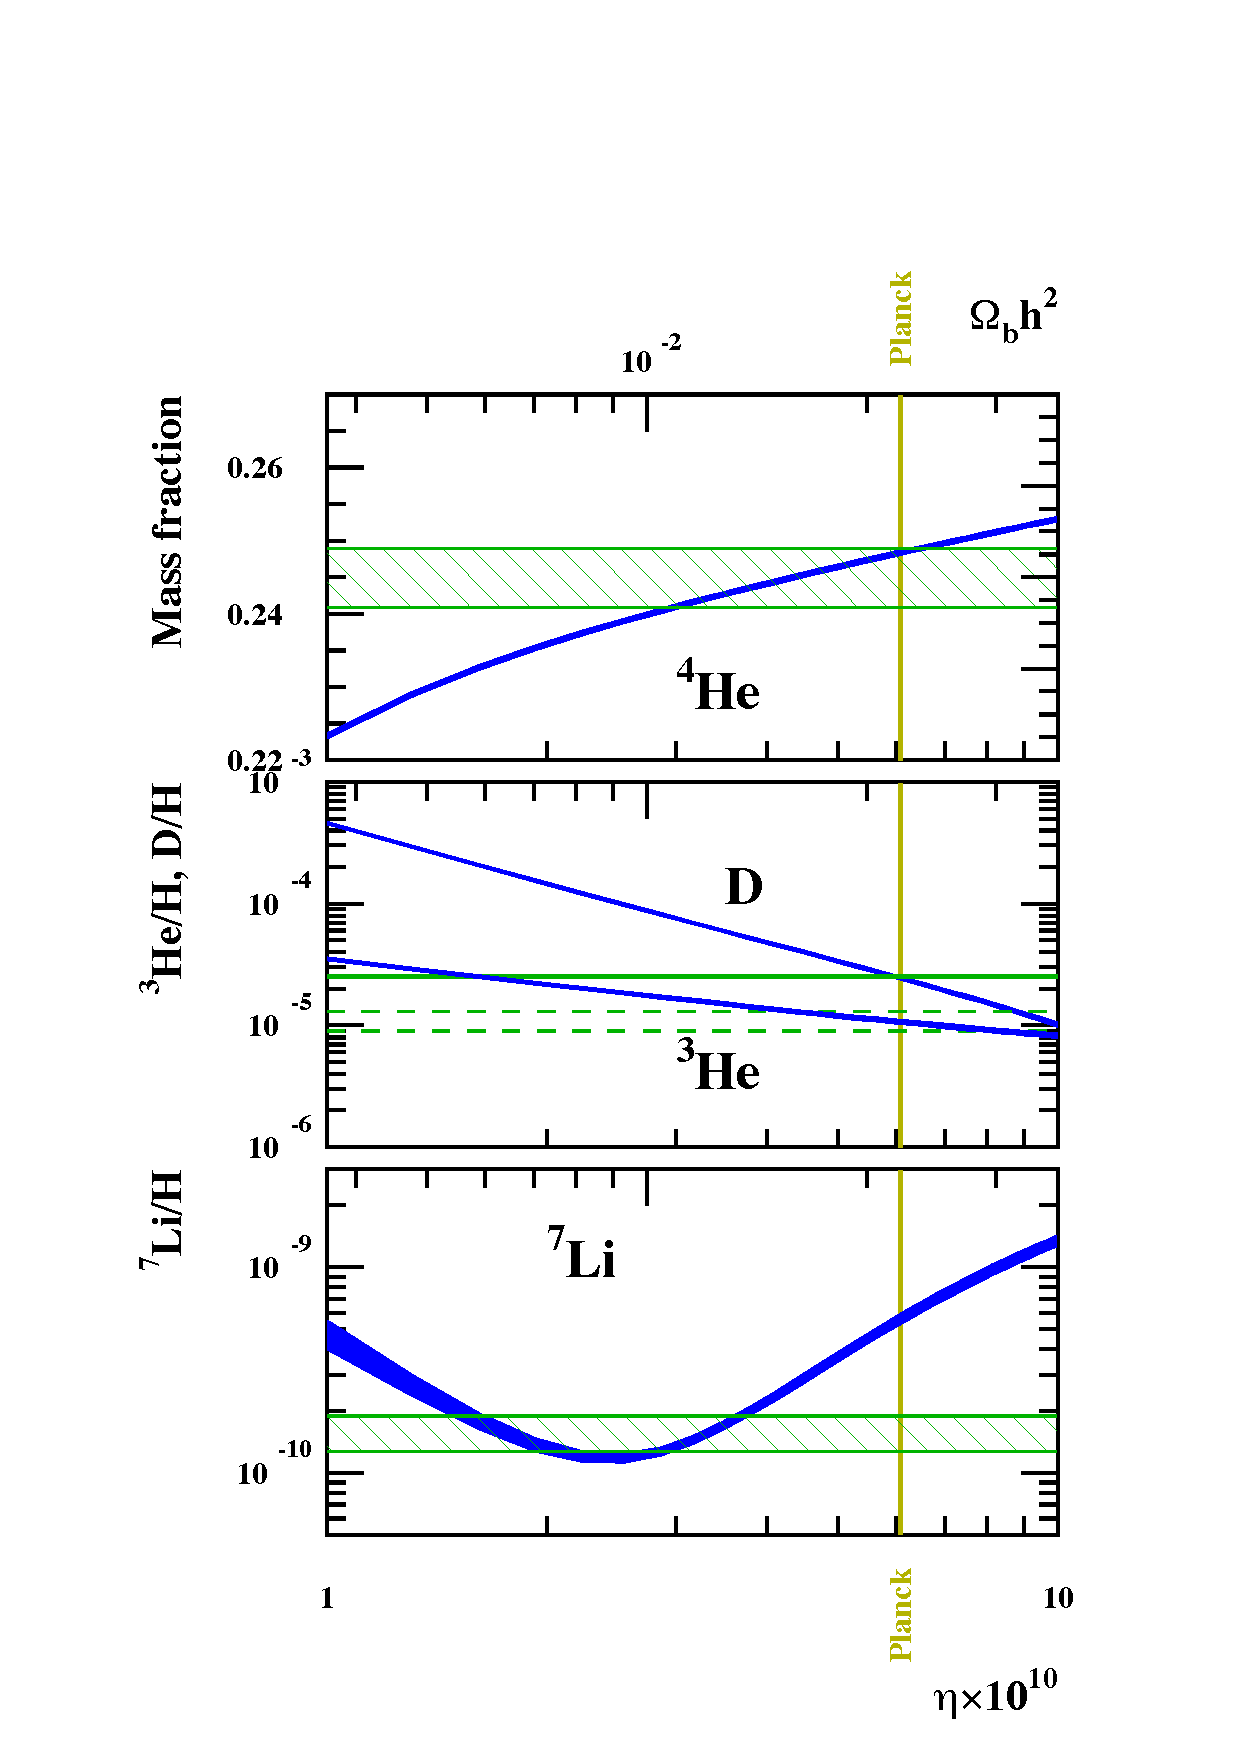
\includegraphics[width=\textwidth]{Intro-FIGS/heli2015.pdf}
\caption[BBN predictions for primordial abundances. Image Credit: \cite{2017-Abundances-Fig}]{BBN predictions for primordial abundances for $^4$He (mass fraction), D, $^3$He, and $^7$Li as a function of the baryon over photon ration, $\eta$, or the baryon density of the Universe, $\Omega_b h^2$. The vertical line comes from the Planck Collaboration measurements for $\Omega_b h^2$ presented in \cite{planck2013}; while the horizontal strips are from primordial abundances presented in \cite{2015-Abundances-Data}. Image Credit: \cite{2017-Abundances-Fig}.}
\label{fig:BBN}
\end{center}
\end{figure}

Deuterium is one of the simplest nucleus formed in the very early universe -- composed by a single proton and a single neutron, they are formed via the following reaction: $p + n \rightarrow D + \gamma$. As strong-force interactions govern the formation of deuterium, this is a very energy efficient reaction. Although, at the time of decoupling, since photons are much more abundant than baryons and the energy of some photons was much higher than the baryon's, $E_{\gamma} \geq E_{b}$, deuterium was destroyed by a mechanism called `photo-dissociation' \citep{2000Deuterium-Tyler}. Only when the temperature drops to around $T_D \approx 8\times 10^8$K that the deuterium formation rate wins over the dissociation rate, leading to a neutron-to-proton ratio of $n_n/n_p \approx 1/7$. Right after this period, all free neutrons end up firstly bound in deuterium atoms -- mostly due to the strong-force nature of the interactions.

\qquad With a higher binding energy than that of deuterium, $^4$He then starts forming as soon as the D density is sufficiently high. Having a higher binding energy ensures that helium-4 cannot be destroyed by photons via photo-dissociation. This process transforms almost all D into $^4$He, with the exception of a small fraction of deuterium. Since at this moment almost all neutrons are present in atoms of $^4$He, the number density of such nuclei can be estimated by taking into account the number of free protons after helium is formed: $n_{H} = n_p - n_n$. 

\qquad The `mass fraction Y` of $^4$He of the total baryon density is defined as \citep{2000-BBN-Review,2016R-BBN-Review}:
\begin{align}
    Y & = \frac{4n_{He}}{4n_{He}+n_H} \\
      & = \frac{2n_n}{n_p + n_n} \approx 0.25\, ,
\end{align}
given that the ratio $n_n/n_p \approx 1/7$ at the time deuterium formation ratio has enough temperature to win over photo-dissociation to form helium-4. This result means that at least a quarter of the Universe's baryonic content should be in the form of helium-4 and it is with perfect agreement with observations \citep{2015-Abundances-Data,2017-Abundances-Fig}.

\qquad From Figure \ref{fig:BBN}, one can see that there's a strong dependency between the $^4$He and D abundances and the baryon content of the Universe, $\Omega_b$. With a larger baryon density, two main consequences arise for these two abundances. The first one is that, with a larger baryon-to-photon ratio, deuterium would form much earlier, with fewer neutrons decaying leading to a higher value for Y. The second consequence, in a similar reasoning, would be that deuterium would convert into helium-4 much more efficiently, leading to a much lower fraction of D.

\qquad Lastly, neutrinos play a major role in BBN given the epoch of the 
Universe one considers. At such early times, neutrinos act as relativistic which influence BBN in various ways. As an example, electron neutrinos influence and control the fraction of free neutrons available, limiting the formation of primordial $^4$He. The number of active neutrinos, $N_{\nu}$, also change considerably predictions for BBN abundances. If $N_{\nu} > 3$, fewer neutrons would decay, resulting in a much higher helium-4 abundance \citep{2007Steingman-BBN}.


% \begin{itemize}
% \item characteristics of the Euclid mission
% \item Description of euclid's observational strategy 
% \item Euclid's Impact in the future of cosmology
% \item Euclid as a cross-correlation's machine
% \end{itemize}

%%%%%%%%%%%%%%%%%%%%%%%%%%%%%%%%%%%%%%%%%%%%%%%%%%%%%%%%%%%
%   				THESIS STRUCTURE
%%%%%%%%%%%%%%%%%%%%%%%%%%%%%%%%%%%%%%%%%%%%%%%%%%%%%%%%%%%
\section{Thesis Structure}
\label{sec:intro:structure}
At last, I outline here the structure of chapters to come together with the list of authors and collaborators in the published and to be published papers related to the work presented in each chapter.

\textbf{Chapter \ref{Chap:BOSS}}: \textit{Tomographic Analysis of BOSS DR12 Galaxy Clustering in Harmonic Space} \\[0.6em]
In this following chapter, I present the work I have done performing an angular power spectrum analysis of BOSS Large Scale Structure galaxy catalogue from \cite{BOSSCatalogue2016}. In this work, I depart from the official LSS BOSS catalogues and masks. I then proceed to build up the full schema in order to extract cosmological information using a harmonic decomposition framework: galaxy maps and masks, angular power spectra measurements with a Pseudo-$C_{\ell}$ estimator, the theoretical $C_{\ell}$ formalism, and construction and validation of a covariance matrix. Finally, in order to assess the viability of using the full shape of the angular power spectra for a cosmological analysis, I have performed systematic contamination null-tests to ensure the measured $C_{\ell}$s were clean from any sort of photometric and observational effects.

\qquad This work, presented in \cite{2018LoureiroBOSS}, has been accepted for publication by Monthly Notices of the Royal Astronomical Society (MNRAS) and it was performed in collaboration with Bruno Moraes, Andrei Cuceu, Michael McLeod, Lorne Whiteway, Sreekumar T. Balan, Aur\'elien Benoit-L\'evy, Ofer Lahav, Marc Manera, Richard Rollins, and Henrique S. Xavier.

\bigskip

\textbf{Chapter \ref{Chap:BOSS-Cosmo}}: \textit{Cosmological Measurements from Angular Power Spectra Analysis of BOSS DR12 Tomography} \\[0.6em]
 In this Chapter, I outline the procedures and formalism to perform a Bayesian analysis for cosmological inference using measurements of the angular power spectra. I then proceed to perform high level consistency checks on the angular power spectra measurements produced in Chapter \ref{Chap:BOSS}, as well as consistency checks on the cosmological inference pipeline and the covariance matrices produced for and with the BOSS-$C_{\ell}$s. Finally, when combining this new BOSS data vectors with CMB data from the Planck experiment and the JLA SNe Ia compilation data-set, I demonstrate that extremely competitive cosmological constraints can be obtained from a large scale structure analysis of spectroscopic galaxies in Harmonic Space. 

\qquad This work, also presented in \cite{2018LoureiroBOSS}, has been accepted by Monthly Notices of the Royal Astronomical Society (MNRAS) and it was performed in collaboration with Bruno Moraes, Andrei Cuceu, Michael McLeod, Lorne Whiteway, Sreekumar T. Balan, Aur\'elien Benoit-L\'evy, Ofer Lahav, Marc Manera, Richard Rollins, and Henrique S. Xavier.

\bigskip

\textbf{Chapter \ref{Chap:Neutrinos}}: \textit{Neutrino Masses from Combined Cosmological Probes and Oscillation Experiments' Constraints} \\[0.6em]
In this follow-up chapter, I investigate the impact of several neutrino mass models in the determination of the upper bound of the sum of neutrino masses, $\sum m_{\nu}$. I demonstrate that a physically motivated model, which takes into account constraints from particle physics experiments, can not only yield robust constraints on \NM{} when compared to usual cosmological approximation but also to set an upper bound to the mass of the lightest neutrino mass. This analysis was performed using the BOSS data vector in harmonic space in combination with Planck CMB and Lensing, SNe Ia from the Pantheon compilation, and BBN data from deuterium-to-hydrogen fraction.

\qquad This work, presented in \cite{2018LoureiroNeutrinos}, has been submitted to Physical Review Letters (PRL) and it was performed in collaboration with  Andrei Cuceu, Bruno Moraes, Lorne Whiteway, Michael McLeod, Sreekumar T. Balan, Aur\'elien Benoit-L\'evy, Ofer Lahav, Marc Manera, Richard Rollins, and Henrique S. Xavier.

\bigskip

\textbf{Chapter \ref{Chap:BPL}}: \textit{An investigation of Bayesian Angular Power Spectra Estimators applied to Galaxy Clustering} \\[0.6em]
The main goal of this chapter was to test, and benchmark a general Bayesian angular power spectra estimator for data distributed on a sphere with a final goal of being a part of the official Euclid $C_{\ell}$ estimator pipelines. The method was originally developed to be applied to CMB temperature, CMB polarisation modes by \cite{SreeThesis}. In this chapter I perform the necessary adaptations to investigate an application of the method to galaxy clustering -- with a future goal to extend it to weak lensing convergence ($\kappa$), cosmic shear ($\gamma_1$ \& $\gamma_2$), and cross-correlations of all previous probes. I perform a series of tests related to the impact of the survey's geometry in the spherical harmonics and its impact in the estimated angular power spectra of galaxies. Finally, I produce and test the method in Euclid-like log-normal simulations for two contrasting noise scenarios, demonstrating that the ideal way to deal with the noise in the case of galaxy clustering is to treat it as anisotropic.

\qquad This is an investigatory chapter with preliminary results. Extending this work to the point of completion is one of the objetives on my work as an Euclid Research Assistance in the next year. This work is in preliminary preparation to be submitted to MNRAS and it was performed in collaboration with Sreekumar T. Balan, Lorne Whiteway, Andrei Cuceu, Lee Whittaker, and Malak Olamaie.

\bigskip

\textbf{Chapter \ref{Chap:Conclusions}}: \textit{Final Considerations, Conclusions \& Future Prospects} \\[0.6em]
I finalise this work by highlighting some key points learned from performing this extensive analysis of the BOSS data release 12 spectroscopic data-set and the resulting cosmological findings. Here I point out my contributions to the narrow field of using spherical harmonics to study and understand the large scale structure of galaxies in the Universe and its cosmological implications not only for cosmology but also for neutrino physics. Moving on, I comment on future prospects of my work, natural extensions of it, and a 5 year broad plan for future research and contributions.

% \textbf{Chapter \ref{sec:conclusion}} \\[0.2em]
% \blindtext
